\documentclass[aps,prx,reprint,longbibliography]{revtex4-2}

\usepackage[T1]{fontenc}
\usepackage[utf8]{inputenc}
\usepackage{lmodern,amsmath,amssymb,bm,array,booktabs,longtable,mathrsfs,mathtools,microtype}
\usepackage{graphicx,tikz}
\usetikzlibrary{arrows.meta,calc,positioning,shapes.geometric}
\usepackage{xurl}
\usepackage[hidelinks]{hyperref}
\pdfstringdefDisableCommands{\def\\{ }}
\setlength{\emergencystretch}{1.5em}
\allowdisplaybreaks[1]
\clubpenalty=10000
\widowpenalty=10000
\displaywidowpenalty=10000
\raggedbottom
\providecommand{\I}{I}
\providecommand{\Tr}{\operatorname{Tr}}
\providecommand{\tr}{\operatorname{tr}}
\providecommand{\trn}{\operatorname{tr}_0}
\providecommand{\Phis}{\Phi_{\rm ret}}
\providecommand{\diag}{\operatorname{diag}}
\providecommand{\Var}{\operatorname{Var}}
\providecommand{\Cov}{\operatorname{Cov}}
\providecommand{\E}{\mathbb E}
\providecommand{\dd}{\mathrm d}
\providecommand{\Fret}{F_{\rm ret}}
\providecommand{\hnu}{h_\nu}
\providecommand{\Mpl}{M_{\rm Pl}}
\providecommand{\SI}{Supplemental Material}
\providecommand{\spec}{\operatorname{spec}}
\providecommand{\rank}{\operatorname{rank}}
\providecommand{\Herm}{\operatorname{Herm}}
\providecommand{\Hom}{\operatorname{Hom}}
\providecommand{\ii}{\mathrm i}
\providecommand{\R}{\mathbb R}
\providecommand{\C}{\mathbb C}
\providecommand{\HH}{\mathbb H}
\providecommand{\RP}{\mathbb{RP}}
\providecommand{\CP}{\mathbb{CP}}
\providecommand{\HP}{\mathbb{HP}}
\providecommand{\norm}[1]{\left\lVert#1\right\rVert}
\newcolumntype{L}[1]{>{\raggedright\arraybackslash}p{#1}}
\definecolor{direction}{RGB}{26,103,134}
\definecolor{plane}{RGB}{127,65,125}
\definecolor{reference}{RGB}{72,86,98}
\hypersetup{pdftitle={Physics Without an Outside Observer: A Finite Geometry, Broken and Completed},pdfauthor={Yongzi CHEN},pdfsubject={Five postulates, finite comparison, breaking and completion}}


\begin{document}

\title{Physics Without an Outside Observer:\\ A Finite Geometry, Broken and Completed}
\author{Yongzi CHEN}
\email{23103646d@connect.polyu.hk}
\affiliation{Department of Physics and Materials, The Hong Kong Polytechnic University, Hung Hom, Kowloon, Hong Kong, China}
\begin{abstract}
What cannot be observed is not described; only a universal rule is a law. These rules give three postulates of equality and two of existence. The first three fix four complex amplitudes and five directions of distinction in a finite geometry of relations without succession. Multiplying one side of a division by $i$ preserves the positive norm and reverses its metric signs. The other two break this equality: a world line takes a direction, and its encounters are common to all participants. Completing the breaking gives the dynamics: a determinant law in one complex variable. Normalized Ihara--Bass reduction recovers the original disagreement operator plus a scalar. Two successive steps give a clock and spacetime with one time and three space directions. Completing the four divisions gives Standard Model gauge fields and three families of matter. A source received by another line gives interaction; returned to its own past, rest mass. Transport of the whole frame gives Einstein--Cartan gravity with a positive cosmological constant; its charge is the complete rest energy. The history needed to compare whole frames determines gravity's weakness. Laws and constants emerge together in a long wavelength action, with the electron rest energy setting the unit.
\end{abstract}
\maketitle

\section{The method}
\label{sec:method}

We use two rules: \emph{what cannot be observed is not described; only a universal rule is a law}.

Imagine a cat that observes the world and can never be observed. The world makes no response by which its presence can be distinguished. Studying this cat and leaving it alone give exactly the same account. We therefore leave it out: within our system, that cat does not exist.

Two frogs sit on opposite banks. Their places distinguish them. Counting two occupants distinguishes two from one. When no possible comparison separates the supposed two, we have named one frog twice. The smallest observation is one distinction.

An outside observer would supply a stage, axes, a clock, probabilities, names, and a zero. Each must be supplied by systems within the account. Physics has repeatedly removed a privileged reference: Copernicus displaced the Earth from the centre, Galileo made uniform motion relative, and Einstein removed absolute time~\cite{Copernicus,Galileo,Einstein1905}. Here the two rules remove the privileged observer and the difference in standing between observing and being observed.

Newton's Rule II assigns, as far as possible, the same causes to natural effects of the same kind; his Rule III extends experimentally universal qualities to all bodies~\cite{Newton}. Our second rule gives every observer equal standing in an elementary comparison, including one's own past. Every observer can itself be observed, so observing and being observed have equal standing.

An encounter must be the same encounter for every participant. Each describes it in its own frame; their completed comparison is common to them. An existing system makes one unit distinction at each moment and compares itself with its preceding moment. An immediate reversal erases the distinction just made. These requirements give five postulates: three of equality and two of existence.

The first three fix a geometry containing relations and no succession. The last two select a world line whose actual direction breaks the equality of its possibilities. We complete this breaking wherever the geometry allows it. The allowed closed histories give a determinant law; this is the dynamics. Two successive steps then supply a clock and spacetime. Fields, matter, mass and gravity follow as the completion proceeds through the four divisions. Each quantity receives its physical name as it appears and enters the next step with its law and its constants. The observer finds within this physics the standards it uses to describe the world.

\section{The five postulates}
\label{sec:postulates}

A system is whatever compares or is compared. The first three postulates express relativity; the last two express existence. We write the antiunitary pairing of observing with being observed as $\Theta=JK$, where $K$ is complex conjugation and $J$ is unitary; P3 gives its square.

\paragraph*{P1. There is no outside observer.}
An elementary system has a finite complex Hilbert space $H$; a pair has $H\otimes H$. Pure states are rays. A mixed state $\rho$ is positive with $\Tr\rho=1$, and a complete set of outcomes has positive effects $F_a$ with
\begin{equation}
 p(a\mid\rho)=\Tr(\rho F_a),\qquad \sum_aF_a=I.
 \label{eq:probability}
\end{equation}
Every reference in this pairing is another system in the account.

\paragraph*{P2. All inside observers have equal standing, including one's own past.}
The comparison is invariant under exchange, a common unitary frame change preserving P3, and symplectic transposition on either operator factor. Its symplectic transposition is
\begin{equation}
 X^\sharp=\Theta X^\dagger\Theta^{-1}=JX^{\mathsf T}J^{-1}.
 \label{eq:sharp}
\end{equation}
Comparison with one's earlier state has the same form as comparison with another participant.

\paragraph*{P3. Observing and being observed have equal standing.}
There is an antiunitary $\Theta$ with $\Theta^2=-I$. The entire nonzero real space of elementary distinctions is
\begin{align}
 \mathscr Q&=\{a=a^\dagger:\Tr a=0,\ [a,\Theta]=0\}\ne\{0\},\notag\\
 a^2&=\trn(a^2)I\quad(a\in \mathscr Q),\qquad
 \trn=\Tr/\dim_\C H.
 \label{eq:postulate-square}
\end{align}
The scalar-square condition applies to the whole space $\mathscr Q$. Every nonzero distinction has two eigenvalues of equal magnitude and opposite sign.

\paragraph*{P4. One encounter is the same for every observer.}
Local frames are compared by reciprocal unitary transport:
\begin{equation}
 U_{yx}=U_{xy}^{-1},\qquad
 U_{xy}\mapsto g_xU_{xy}g_y^{-1}.
 \label{eq:transport}
\end{equation}
A complete encounter contracts its endpoint states with the transport, or takes a trace around a closed history. Where a compass points changes with its frame; the angle between the compass brought home around a circuit and the one left there is a fact.

\paragraph*{P5. Existence is a world line.}
A system takes one unit distinction at each moment and compares itself with its preceding moment. In a local orthonormal frame $\{a_t^{(m)}\}$ of $\mathscr Q$,
\begin{equation}
 \Psi_{m+1}=(a_{t_m}^{(m)}\otimes I)\Psi_m,
 \qquad t_{m+1}\ne t_m.
 \label{eq:postulate-step}
\end{equation}
The direction labels are compared by the transport of P4. The frog jumps at each moment, does not jump straight back, and carries its previous jump itself.

\section{The geometry}
\label{sec:geometry}

We first apply P1--P3. A rotation of distinctions must preserve their two opposite values throughout $\mathscr Q$. This fixes the dimension before a succession of comparisons is introduced.

\subsection{Four amplitudes and five directions}

The vector $\Theta v$ is perpendicular to $v$ and has the same length. Thus $H$ is a quaternionic space $\HH^n$, or $\C^{2n}$. Distinctions are its traceless quaternionic Hermitian matrices. For $n=1$, their space is zero. For $n\geq3$, $\diag(1,-1,0,\ldots)$ violates Eq.~\eqref{eq:postulate-square}. For $n=2$, every distinction is
\begin{equation}
 \begin{gathered}
 a=\begin{pmatrix}r&q\\\bar q&-r\end{pmatrix},\qquad
 a^2=(r^2+|q|^2)I,\\
 r\in\R,\qquad q\in\HH.
 \end{gathered}
 \label{eq:quaternionic}
\end{equation}
It has five real components. Consequently
\begin{equation}
 H=\C^4\simeq\HH^2,\qquad \mathscr Q\simeq\R^5.
 \label{eq:four-five}
\end{equation}
Polarizing the square gives the Clifford relation. In an oriented orthonormal frame,
\begin{equation}
 \gamma_s\gamma_t+\gamma_t\gamma_s=2\delta_{st}I,
 \qquad \gamma_1\gamma_2\gamma_3\gamma_4\gamma_5=I.
 \label{eq:clifford}
\end{equation}
For a direction $v$, we write $\gamma(v)=\sum_t v_t\gamma_t$.
The common rotations form $Sp(2)=Spin(5)$. The vectors paired by $\Theta$ lie in the same eigenspace of any distinction that commutes with $\Theta$; each side is a quaternionic line.

\subsection{Agreement belongs to the pair}

The invariant contractions determine the comparison. In a complex orthonormal basis $u_j$, let
\begin{equation}
 \begin{gathered}
 \Omega=\frac12\sum_{j=1}^4u_j\otimes\Theta u_j,\qquad
 E_\Omega=4|\Omega\rangle\langle\Omega|,\\
 P(x\otimes y)=y\otimes x.
 \end{gathered}
 \label{eq:singlet}
\end{equation}
The invariant operator space is generated by $I,P,E_\Omega$. Symplectic transposition of one factor interchanges $P$ and $E_\Omega$, so P2 gives them equal coefficients. Taking the identity term and the five unit distinctions in their common normalization gives
\begin{equation}
 L=I\otimes I+\sum_{t=1}^5\gamma_t\otimes\gamma_t
   =2(P+E_\Omega).
 \label{eq:comparison}
\end{equation}
The singlet, symmetric, and vector grades have dimensions one, ten, and five. The sixteen even Clifford products give an orthonormal pair basis $\lvert S\rangle=(\gamma_S\otimes I)\Omega$, with $|S|=0,2,4$. For $N\lvert S\rangle=|S|\lvert S\rangle$,
\begin{equation}
 \begin{gathered}
 L=6I-2N,\qquad L\Omega=6\Omega,\\
 \spec L=\{6^{(1)},2^{(10)},-2^{(5)}\}.
 \end{gathered}
 \label{eq:spectrum}
\end{equation}
The difference from complete agreement is
\begin{equation}
 \begin{gathered}
 \Delta=6I-L
 =\frac12\sum_t(\gamma_t\otimes I-I\otimes\gamma_t)^2\geq0,\\
 \ker\Delta=\C\Omega.
 \end{gathered}
 \label{eq:disagreement}
\end{equation}
The five pair operators $\gamma_t\otimes\gamma_t$ commute: the two minus signs from exchanging distinct generators cancel. Their common agreement therefore belongs to one vector of the pair space. Each of its reduced matrices is $I/4$. For every product state and every convex mixture of product states, $\langle\Delta\rangle\geq4$. Complete agreement lies in the pair relation.

For any unitary $U$, the two reduced matrices of $(U\otimes I)\Omega$ remain $I/4$. Nevertheless $(\gamma_h\otimes I)\Omega$ is perpendicular to $\Omega$, since $\Tr\gamma_h=0$. An unchanged separate description can accompany a changed pair relation.

\subsection{A sign and its square root}

Divide the six-dimensional antisymmetric pair space and reverse the sign on one part. Equal endpoint factors must reproduce that reversal, while conjugate endpoint factors preserve the positive norm. These are two products of one factor.

Put $\Omega_t=(\gamma_t\otimes I)\Omega$. The normalized Pfaffian is
\begin{equation}
 p\!\left(\xi_0\Omega+\sum_t \xi_t\Omega_t\right)
 =\xi_0^2-\sum_t \xi_t^2.
 \label{eq:pfaffian}
\end{equation}
It is positive on the real six-space
$\mathscr V=\operatorname{span}_{\R}\{\Omega,i\Omega_1,\ldots,i\Omega_5\}$.
The action of $SU(4)$ on $\mathscr V$ gives the double cover $SU(4)\to SO(6)$.

For a real subspace $D\subset\mathscr V$, let $P_D$ be its orthogonal projector and $\theta_D=I-2P_D$. A factor depending only on the division is scalar on its two parts. Writing it as $q=\alpha I+\beta\theta_D$, the equation $q^{\mathsf T}q=\theta_D$ gives $\alpha^2+\beta^2=0$ and $2\alpha\beta=1$. One solution is
\begin{equation}
 q_D=I-P_D+iP_D,\quad
 q_D^\dagger q_D=I,\quad q_D^{\mathsf T}q_D=I-2P_D.
 \label{eq:half}
\end{equation}
The Hermitian product on $D$ multiplies $-i$ by $i$ and gives $+1$; the bilinear product multiplies $i$ by $i$ and gives $-1$. A nontrivial division has the four sign-only alternatives $\pm q_D,\pm\bar q_D$.

Up to exchanging its parts, a real six-space has four division types. In $d|6-d$ we call the side of dimension $d\leq3$ the divided side. The dimensions of the rotations within and between the parts are $\binom d2+\binom{6-d}2$ and $d(6-d)$:
\begin{center}\small
\begin{tabular}{@{}cccc@{}}
\toprule
Type&Within&Between&Spin cover\\\midrule
$0\mid6$&15&0&$SU(4)$\\
$1\mid5$&10&5&$SU^*(4)$\\
$2\mid4$&7&8&$SU(2,2)$\\
$3\mid3$&6&9&$SL(4,\R)$\\\bottomrule
\end{tabular}
\end{center}
For $d>0$, the projective null set has the form
\begin{equation}
 \bigl(S^{d-1}\times S^{5-d}\bigr)/\mathbb Z_2,
 \qquad\text{tangent signature }(d-1,5-d).
 \label{eq:nullspace}
\end{equation}
Thus $2\mid4$ has a four-dimensional null tangent space of signature $(1,3)$. Its compact preserving group $SO(2)\times SO(4)$ is the only one in the table with a continuous centre, the rotation of the two-plane. All of these are relations in the geometry. P4 and P5 now give them a succession.

\begin{figure}[tb]
\centering
\resizebox{\columnwidth}{!}{%
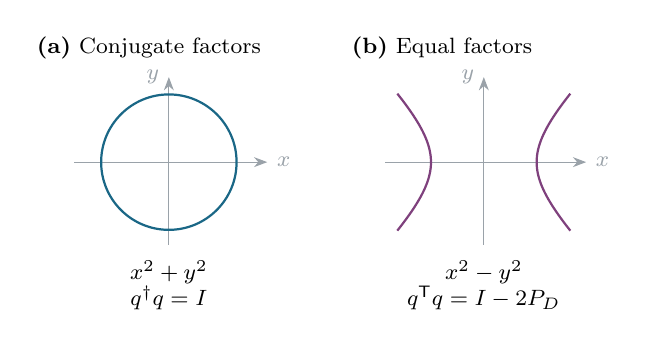
\begin{tikzpicture}[x=1cm,y=1cm,>=Stealth,font=\footnotesize]
\node[anchor=west] at (0,3.0) {\textbf{(a)} Conjugate factors};
\node[anchor=west] at (4.0,3.0) {\textbf{(b)} Equal factors};
\begin{scope}[shift={(1.8,1.55)}]
\draw[->,reference!55] (-1.2,0)--(1.25,0) node[right] {$x$};
\draw[->,reference!55] (0,-1.05)--(0,1.08) node[left] {$y$};
\draw[direction,thick] (0,0) circle(.86);

\node[below,align=center] at (0,-1.13) {$x^2+y^2$\\$q^\dagger q=I$};
\end{scope}
\begin{scope}[shift={(5.8,1.55)}]
\draw[->,reference!55] (-1.25,0)--(1.3,0) node[right] {$x$};
\draw[->,reference!55] (0,-1.05)--(0,1.08) node[left] {$y$};
\draw[plane,thick,domain=-.87:.87,samples=45] plot ({sqrt(.45+\x*\x)},\x);
\draw[plane,thick,domain=-.87:.87,samples=45] plot ({-sqrt(.45+\x*\x)},\x);
\node[below,align=center] at (0,-1.13) {$x^2-y^2$\\$q^{\mathsf T}q=I-2P_D$};
\end{scope}
\end{tikzpicture}}
\caption{The factor $q_D$ sends $(x,y)$ to $(x,iy)$ when $y$ lies in $D$. Conjugate factors preserve the circle of fixed norm; equal factors give the signed form with a hyperbolic positive level set.}
\label{fig:half}
\end{figure}


\section{The breaking and its completion}
\label{sec:breaking}

\begin{figure*}[t]
\centering
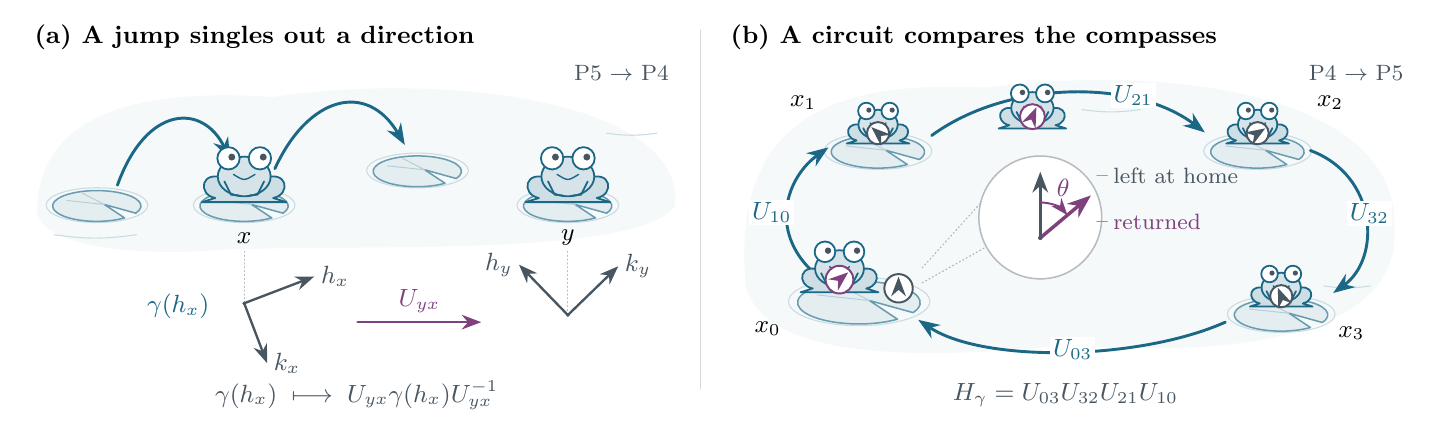
\begin{tikzpicture}[x=1cm,y=1cm,>=Stealth,font=\small,
  line cap=round,line join=round]
% The drawing is 17.6 x 4.85 cm. All glyphs are local to this figure.
\path[use as bounding box] (0,-.2) rectangle (17.6,4.65);
\tikzset{trip/.style={->,direction,line width=1.05pt},
  frame/.style={->,reference,line width=.85pt},
  ripple/.style={direction!23,line width=.4pt}}
\newcommand{\lilypadA}[3]{\begin{scope}[shift={(#1,#2)},scale=#3]
  \draw[ripple] (0,-.04) ellipse (.76 and .26);
  \path[draw=direction!65,fill=direction!12,line width=.55pt]
    (.11,-.03)--(.58,-.16) arc[start angle=-28,end angle=309,x radius=.66,y radius=.23]--cycle;
  \draw[direction!32,line width=.35pt] (-.45,.03)--(.11,-.03)--(-.22,.14);
\end{scope}}
\newcommand{\frogA}[3]{\begin{scope}[shift={(#1,#2)},scale=#3]
  \path[draw=direction,fill=direction!22,line width=.65pt]
    (-.22,-.03) .. controls (-.53,.10) and (-.57,-.22) .. (-.35,-.26)
    --(-.51,-.31)--(-.16,-.31)--(.16,-.31)--(.51,-.31)--(.35,-.26)
    .. controls (.57,-.22) and (.53,.10) .. (.22,-.03);
  \filldraw[draw=direction,fill=direction!18,line width=.65pt] (0,0) ellipse (.32 and .24);
  \filldraw[draw=direction,fill=white,line width=.65pt] (-.19,.22) circle (.135);
  \filldraw[draw=direction,fill=white,line width=.65pt] (.19,.22) circle (.135);
  \fill[reference] (-.15,.235) circle (.042);
  \fill[reference] (.23,.235) circle (.042);
  \draw[direction,line width=.5pt] (-.13,.025) .. controls (0,-.055) .. (.13,.025);
  \draw[direction,line width=.65pt] (-.24,-.06)--(-.16,-.22)--(-.06,-.23);
  \draw[direction,line width=.65pt] (.24,-.06)--(.16,-.22)--(.06,-.23);
\end{scope}}
\newcommand{\dialA}[5]{\begin{scope}[shift={(#1,#2)},scale=#3]
  \filldraw[white,draw=#5,line width=.7pt] (0,0) circle (.22);
  \draw[->,#5,line width=.9pt] (0,0)--(#4:.18);
  \fill[#5] (0,0) circle (.022);
\end{scope}}

\node[anchor=west,font=\bfseries\small,inner sep=0] at (.08,4.53)
  {(a) A jump singles out a direction};
\node[anchor=east,text=reference,font=\footnotesize,inner sep=0] at (8.15,4.08)
  {P5 $\rightarrow$ P4};
\node[anchor=west,font=\bfseries\small,inner sep=0] at (8.92,4.53)
  {(b) A circuit compares the compasses};
\node[anchor=east,text=reference,font=\footnotesize,inner sep=0] at (17.48,4.08)
  {P4 $\rightarrow$ P5};
\draw[reference!22] (8.55,.06)--(8.55,4.62);

% (a) The jumper arrives at x; y is the second participant, off the jump path.
\path[fill=direction!4] (.12,2.40)
  .. controls (.20,3.61) and (1.51,3.88) .. (3.11,3.77)
  .. controls (5.21,4.09) and (8.37,3.75) .. (8.22,2.38)
  .. controls (7.74,1.73) and (4.25,1.90) .. (2.49,1.83)
  .. controls (1.13,1.72) and (.03,1.93) .. cycle;
\draw[ripple] (.34,2.02) to[bend right=8] (1.38,2.02);
\draw[ripple] (7.35,3.31) to[bend right=8] (7.99,3.31);
\lilypadA{.88}{2.43}{.85}
\lilypadA{2.75}{2.43}{.85}
\lilypadA{4.95}{2.87}{.85}
\lilypadA{6.86}{2.43}{.85}
\draw[trip] (1.14,2.65) .. controls (1.51,3.68) and (2.23,3.69) .. (2.57,2.98);
\draw[trip] (3.14,2.86) .. controls (3.56,3.78) and (4.31,3.98) .. (4.79,3.16);
\frogA{2.75}{2.76}{1.05}
\frogA{6.86}{2.76}{1.05}
\node[inner sep=1pt] at (2.75,1.98) {$x$};
\node[inner sep=1pt] at (6.86,1.98) {$y$};
% Each local frame is attached to its own participant, with no pond axes.
\draw[reference!40,densely dotted] (2.75,1.81)--(2.75,1.15);
\draw[reference!40,densely dotted] (6.86,1.81)--(6.86,1.00);
\fill[reference] (2.75,1.15) circle (.025);
\fill[reference] (6.86,1.00) circle (.025);
\draw[frame] (2.75,1.15)--(3.64,1.49) node[right,inner sep=2pt] {$h_x$};
\draw[frame] (2.75,1.15)--(3.04,.39) node[right,inner sep=2pt] {$k_x$};
\draw[frame] (6.86,1.00)--(6.24,1.64) node[left,inner sep=2pt] {$h_y$};
\draw[frame] (6.86,1.00)--(7.50,1.62) node[right,inner sep=2pt] {$k_y$};
\node[text=direction,anchor=east,inner sep=1pt] at (2.35,1.11) {$\gamma(h_x)$};
\draw[->,plane,line width=.9pt] (4.19,.91)--(5.76,.91)
  node[midway,above=2pt,inner sep=1pt] {$U_{yx}$};
\node[text=reference,inner sep=0] at (4.18,-.02)
  {$\gamma(h_x)\;\longmapsto\;U_{yx}\gamma(h_x)U_{yx}^{-1}$};

% (b) An asymmetric, directed pond circuit; labels sit outside its pads.
\path[fill=direction!4] (9.12,1.36)
  .. controls (8.90,3.68) and (10.49,3.97) .. (12.18,3.89)
  .. controls (14.51,4.20) and (17.44,3.80) .. (17.36,2.09)
  .. controls (17.43,.65) and (15.09,.47) .. (13.22,.62)
  .. controls (10.97,.39) and (9.36,.51) .. cycle;
\draw[ripple] (13.39,3.61) to[bend right=8] (14.13,3.61);
\draw[ripple] (16.46,1.37) to[bend right=8] (17.05,1.37);
\lilypadA{10.56}{1.22}{1.18}
\lilypadA{10.80}{3.12}{.90}
\lilypadA{15.62}{3.12}{.90}
\lilypadA{15.92}{1.05}{.90}
\draw[trip] (9.97,1.55) .. controls (9.40,2.09) and (9.65,2.76) .. (10.17,3.13);
\node[text=direction,inner sep=1pt,fill=white] at (9.45,2.30) {$U_{10}$};
\draw[trip] (11.48,3.28) .. controls (12.45,3.99) and (14.06,4.00) .. (14.95,3.32);
\node[text=direction,inner sep=1pt,fill=white] at (14.04,3.79) {$U_{21}$};
\draw[trip] (16.29,3.09) .. controls (17.15,2.77) and (17.19,1.72) .. (16.58,1.28);
\node[text=direction,inner sep=1pt,fill=white] at (17.04,2.29) {$U_{32}$};
\draw[trip] (15.21,.91) .. controls (14.11,.42) and (12.13,.39) .. (11.31,.94);
\node[text=direction,inner sep=1pt,fill=white] at (13.27,.56) {$U_{03}$};
\node[inner sep=0,anchor=east] at (9.57,.83) {$x_0$};
\node[inner sep=0,anchor=south east] at (10.02,3.61) {$x_1$};
\node[inner sep=0,anchor=south west] at (16.37,3.61) {$x_2$};
\node[inner sep=0,anchor=west] at (16.64,.77) {$x_3$};
% Residents compare locally. Purple dials are held between the traveller's hands.
\frogA{10.80}{3.42}{.78}
\dialA{10.80}{3.31}{.64}{138}{reference}
\frogA{15.62}{3.42}{.78}
\dialA{15.62}{3.31}{.64}{32}{reference}
\frogA{15.92}{1.35}{.78}
\dialA{15.92}{1.24}{.64}{112}{reference}
\frogA{12.76}{3.63}{.84}
\dialA{12.76}{3.52}{.72}{67}{plane}
\frogA{10.31}{1.59}{.97}
\dialA{10.31}{1.45}{.80}{40}{plane}
\dialA{11.06}{1.34}{.82}{90}{reference}
% The magnification is linked to the two physical compasses on the home pad.
\draw[reference!45,densely dotted] (11.36,1.41)--(12.27,1.92);
\draw[reference!45,densely dotted] (11.36,1.60)--(12.27,2.61);
\filldraw[fill=white,draw=reference!40,line width=.55pt] (12.86,2.24) circle (.78);
\draw[->,reference,line width=1pt] (12.86,1.98)--(12.86,2.82);
\draw[->,plane,line width=1.25pt] (12.86,1.98)--++(40:.84);
\fill[reference] (12.86,1.98) circle (.028);
\draw[plane,->,line width=.7pt] (12.86,2.43) arc[start angle=90,end angle=40,radius=.45];
\node[text=plane,inner sep=0] at (13.15,2.62) {$\theta$};
\node[anchor=west,text=reference,font=\footnotesize,inner sep=0] at (13.78,2.77) {left at home};
\draw[reference!55,line width=.45pt] (13.71,2.77)--(13.58,2.77);
\node[anchor=west,text=plane,font=\footnotesize,inner sep=0] at (13.78,2.19) {returned};
\draw[plane!65,line width=.45pt] (13.71,2.19)--(13.58,2.19);
\node[text=reference,inner sep=0] at (13.18,-.02)
  {$H_\gamma=U_{03}U_{32}U_{21}U_{10}$};
\end{tikzpicture}
\caption{A jump singles out a direction, which participants compare by transporting it between their local frames. A compass carried around the four-pad circuit returns with holonomy $H_\gamma$ and makes an angle $\theta$ with the compass left at home, unchanged by rotations of the local frames.}
\label{fig:frog-scenes}
\end{figure*}

Every lily pad has the same standing. Then a frog jumps. Its arrival distinguishes the direction it came from, and the frog carries that direction into its next jump. Another frog sees the jump from a different orientation. They have witnessed one event; to compare it, the first frog's direction must be expressed in the second frog's frame. Neither frog has been appointed north.

Now each frog carries a compass, with no compass above the pond. A frog takes its compass from pad to pad, comparing it with the compass at each arrival. After a circuit it compares the compass it carried with the one that stayed at the first pad. They can differ by an angle. That angle belongs to the completed circuit (Fig.~\ref{fig:frog-scenes}).

The first scene starts with a continuing world line and completes the comparison at its encounters: P5, then P4. The second starts with local frames and completes their comparison through a continuing world line: P4, then P5. A particular occurrence distinguishes something among equals; its completion makes that occurrence comparable for all its participants. This is the substance of the gauge-field method: a connection compares local frames, and its closed transport measures the field. Here the frame belongs to a participant, and its own steps carry the comparison.

The six-dimensional geometry has four divisions: $0|6$, $1|5$, $2|4$, and $3|3$, with the smaller side divided. Adding or removing a direction changes the division; we call this \emph{vertical} completion. Rotating the frame while preserving the division is \emph{parallel} completion. To introduce the physics step by step, we visit these places in a different order from their dimensions, and complete every one. The world line first changes its directions; then its frame is transported at each fixed division. The detailed derivations follow these eight steps, in the same order, in Part I of the Supplemental Material~\cite{SI}.

\subsection{Vertical}
\label{sec:vertical}
\setcounter{subsubsection}{0}
\renewcommand{\thesubsubsection}{\arabic{subsubsection}}

\subsubsection{One step}
\label{sec:one_step}

The jump carries the previous direction into the next comparison. On the sixteen pair states, written as even subsets $x$ of five directions, $\gamma_s$ changes $x$ to $x\mathbin\triangle g_s$, where $g_s$ contains the four directions other than $s$. Repeating the arrival direction $t$ gives $\gamma_t^2=I$ and erases the two-step distinction. Keeping that direction in the state therefore gives
\begin{equation}
 B(x',s;x,t)=[s\ne t]\,[x'=x\mathbin\triangle g_s].
 \label{eq:B}
\end{equation}
There are eighty directed states and four continuations from each. The underlying Clebsch graph has sixteen vertices and forty edges.

The compass closes this continuation. A closed transport $H_\gamma$ changes by conjugation at its starting point, and P4 gives every cyclic starting point equal standing. A primitive history repeated $j$ times has weight $1/j$. Counting each closed comparison once gives
\begin{equation}
 \begin{split}
 Z(u;U)&=\exp\!\left[\sum_{r\ge1}\frac{u^r}{r}\Tr B[U]^r\right]\\
 &=\prod_{\gamma\ {\rm primitive}}\det(I-u^{|\gamma|}H_\gamma)^{-1}\\
 &=\det(I-uB[U])^{-1}.
 \end{split}
 \label{eq:law}
\end{equation}
The complex variable $u$ carries the weight and phase of one step. Equal unsigned continuations each have weight $1/4$. The series converges for $|u|<1/4$ and the determinant continues it.

Eliminate the remembered direction. The Ihara--Bass identity~\cite{Ihara,Bass,Hashimoto} gives
\begin{align}
 D(u)&=(1-u^2)^{24}\det K(u),\quad D(u)=\det(I-uB),\notag\\
 K(u)&=(1+4u^2)I-uA,\label{eq:bass}\\
 K(u)/u&\simeq(6I-L)+\chi(u)I,\notag\\
 \chi(u)&=\frac1u+4u-5=\frac{(1-u)(1-4u)}u.\label{eq:chi}
\end{align}
Here $A$ is the graph adjacency. Its character transform $\mathscr F_{xS}=(-1)^{|x\cap S|}/4$ takes $A$ to $L-I$. In one step the law has recovered the geometry of comparison, with just one movable origin.

Its three grade factors are
\begin{equation}
 \begin{gathered}
 k_N(u)=1+4u^2-u(5-2N),\\
 D(u)=(1-u^2)^{24}k_0(u)k_2(u)^{10}k_4(u)^5.
 \end{gathered}
 \label{eq:polynomial}
\end{equation}
Resolving the encounter first separates its five channels into $a_+=5-N$ positive and $a_-=N$ negative signs at grade $N$. Its local factor is
\begin{equation}
 (1+u)^{a_+-1}(1-u)^{a_--1}
 \bigl[1+4u^2-u(a_+-a_-)\bigr].
 \label{eq:encounter_first}
\end{equation}
The product over the sixteen states is Eq.~\eqref{eq:polynomial}: each edge factor has total exponent twenty-four. P5 followed by P4 and P4 followed by P5 have given one law.

\subsubsection{Two steps}
\label{sec:two_steps}

The last two jumps meet in the comparison required by P4, while P5 carries their order. One's own past has the equal standing of P2. If $h$ is the last direction and $k$ the preceding one, the comparisons are
\begin{equation}
\begin{gathered}
 r_{m,m}=\Omega,\qquad r_{m,m-1}=(\gamma_h\otimes I)\Omega,\\
 r_{m,m-2}=\pm\lvert hk\rangle.
 \end{gathered}
 \label{eq:three_comparisons}
\end{equation}
Here $r_{a,b}$ compares moments $a$ and $b$ on the line. The frog's last two jumps have supplied a reference, a direction, and a plane. Let $n$ denote the singlet reference direction $\Omega$ in the real six-space. Write $F=\{h,k\}$; its complement $C$ contains the other three vector directions.

Among the rotations preserving a $d|6-d$ division, a continuous centre occurs precisely at $d=2$. The two planes already present above have central rotations
\begin{equation}
 \begin{gathered}
 T_{\rm own}=i\gamma_h,\qquad T_F=\gamma_h\gamma_k,\\
 H_k=\frac{I+i\gamma_k}{\sqrt2},\qquad
 H_kT_{\rm own}H_k^\dagger=T_F.
 \end{gathered}
 \label{eq:clocks}
\end{equation}
Together with $i\gamma_k$ they form a quaternion triple. The central phase compares successive moments while preserving the plane. It is a clock: $\{n,h\}$ reads proper time, and $F$ compares clocks at an encounter.

Here a quantity receives its first physical name, and the name is only a name. The completed derivation gives a consistent reading of this rotation as a clock and of each later quantity as the physical quantity whose form it has. Changing those names changes none of the relations. We use them so that the reader can follow the physics as it appears; the end of this part brings the whole reading together.

For the $2|4$ sign, a null vector has equally long components on its two sides. Dividing out its length gives $(S^1\times S^3)/\mathbb Z_2$, with local conformal metric
\begin{equation}
 ds^2=-d\tau^2+d\Omega_3^2,\qquad
 c=\frac{\Delta x}{\Delta t}.
 \label{eq:spacetime}
\end{equation}
Here $\Delta t$ is the duration of one clock increment and $\Delta x$ its spatial extent on the null comparison. There is one time coordinate and three space coordinates; $c$ converts their units. P4 makes that null encounter the same for every observer.

\subsubsection{Any number of directions}
\label{sec:all_directions}

A continuing line carries its division with it. Adding a direction and removing it have the equal standing of P3, and their comparison must survive the change. On the exterior algebra of the six-space, let $\varepsilon_a$ add direction $a$, $\iota_a$ contract it, and $\Pi_r$ project onto degree $r$. Their completion is
\begin{equation}
 \begin{gathered}
 J_a=\varepsilon_a+\iota_a,\qquad\{J_a,J_b\}=2\delta_{ab}I,\\
 \sum_r\Pi_rJ_aJ_b\Pi_r
 =\varepsilon_a\iota_b-\varepsilon_b\iota_a=T_{ab}\quad(a\ne b).
 \end{gathered}
 \label{eq:vertical}
\end{equation}
Thus the degree-preserving part of two vertical changes is a parallel rotation. Its action is
\begin{equation}
 R_{ab}(\vartheta)=e^{\vartheta J_aJ_b/2},\qquad R_{ab}(2\pi)=-I.
 \label{eq:spin}
\end{equation}
The even vertical algebra acts on the same four amplitudes as the original comparison. In this representation,
\begin{equation}
 \rho_4(J_nJ_t)=-i\gamma_t,\qquad
 \rho_4(J_sJ_t)=\gamma_s\gamma_t\quad(s\ne t).
 \label{eq:vertical_four}
\end{equation}
The five $J_nJ_t$ square to $-I$ and anticommute, just as the five $-i\gamma_t$ do. Thus one original distinction is $\gamma_t=i\rho_4(J_nJ_t)$. A full turn returns a minus sign: the comparison has spin one half.

Each divided direction contributes the factor $i$ of Eq.~\eqref{eq:half}. On a divided set $S$,
\begin{equation}
 z_S=\det q_S=i^{|S|},\qquad u_S=z_S/4,\qquad p_S=(-1)^{|S|}.
 \label{eq:phase}
\end{equation}
The four quarter points are exactly the four divisions. With the side $d\leq3$ divided, they give
\begin{equation}
 \begin{array}{c|rrrr}
 d&0&1&2&3\\\hline
 u_S&1/4&i/4&-1/4&-i/4\\
 \chi(u_S)&0&-5-3i&-10&-5+3i
 \end{array}
 \label{eq:division_values}
\end{equation}
The grade factors at these points follow from Eq.~\eqref{eq:polynomial}.

A return also carries its Clifford sign. Let $A_-$ be the matrix of $\sum_s(\gamma_s\otimes I)$ in the pair basis $\lvert S\rangle$. It has the graph's edges with their Clifford amplitudes; anticommutation gives $A_-^2=5I$. Its diagonal resolvent, with repeated first returns removed, gives
\begin{equation}
\begin{gathered}
 \Phis(z)=-\frac{z^4}{16+3z^2},\\
 \Phis(\pm1)=-\frac1{19},\qquad\Phis(\pm i)=-\frac1{13}.
 \end{gathered}
 \label{eq:signed_first_return}
\end{equation}
The first departure has weight $1/5$, each continuation $1/4$, and $z=4u$ marks the length.

For $r_S$ vector directions in $S$, the returned comparison and the channels across the division are
\begin{equation}
 \begin{gathered}
 L_S=5-r_S+r_Sp_S,\qquad w_S=z_S/L_S,\\
 \Psi_S=-\frac{\Phis(4w_S)}{16w_S^2}
       =\frac{p_S}{L_S^2+3p_S},\\
 t_S=2|w_S|,\qquad r_S^{\rm amp}=1-t_S,\\
 N(S)=|S|(6-|S|)+[|S|\ {\rm odd}].
 \end{gathered}
 \label{eq:support_rule}
\end{equation}
An odd set adds the antilinear channel. Even sets read a Hermitian count; odd sets read an amplitude whose square is a count. In particular, the even plane and its odd colour lift have responses $1/28$ and $1/2$. The norm-preserving directed step is $\mathcal U=(2/5)B-(3/5)\mathcal R_{\rm edge}$, where $\mathcal R_{\rm edge}$ reverses an edge. Its transmission and reflection, and those at a single vector direction, are
\begin{equation}
 t_0=\frac25,\quad r_0=\frac35,\qquad
 t_{\rm v}=\frac23,\quad r_{\rm v}=\frac13.
 \label{eq:grade_amplitudes}
\end{equation}
They are the successive reciprocals and ratios of $k_0,k_2,k_4$ at the plane's quarter point.

\subsubsection{The critical step}
\label{sec:critical}

At $u=1/4$ the singlet factor has a simple zero. The symmetric and vector roots have modulus $1/2$; all other noncritical roots have modulus one. A continuing line can therefore meet its own past through a response of infinite range at this one zero.

The return includes every intermediate comparison. Let $N_{\rm ret}$ count its steps, and let $n_L,n_F$ count visits to the vector ($|S|=4$) and symmetric ($|S|=2$) pair states. Marking them by $z,x,y$ gives
\begin{equation}
\begin{gathered}
 \Fret(z;x,y)=\frac{z^4x^2y(1+zy)}{16-8zy-3z^2xy-3z^3xy^2},\\
 \Fret(z)=\Fret(z;1,1).
 \end{gathered}
 \label{eq:returns}
\end{equation}
Every return closes. Its mean length and sign-reversing probability per continuation are
\begin{equation}
 \Fret(1)=1,\qquad \E N_{\rm ret}=16,\qquad
 a=\frac{1-\Phis(1)}8=\frac5{38}.
 \label{eq:return_numbers}
\end{equation}

A phase $e^{-i\mu}$ on a completed step moves the zero to $u_c=e^{i\mu}/4$. It rotates the pair comparison even while both separate reduced states stay $I/4$:
\begin{equation}
 (e^{-i\mu\gamma_h}\otimes I)\Omega
 =\cos\mu\,\Omega-i\sin\mu\,(\gamma_h\otimes I)\Omega.
 \label{eq:joint_clock}
\end{equation}
A perpendicular translation with phase $k$ completes this moving clock as
\begin{equation}
 U=e^{-ik\gamma_j}e^{-i\mu\gamma_h},\quad j\ne h,
 \qquad\boxed{\cos\omega=\cos\mu\cos k}.
 \label{eq:dispersion}
\end{equation}
It is the cosine rule for a right spherical triangle. Phase per time is energy, phase per distance is momentum, and the phase left at rest is mass:
\begin{equation}
 E=\frac{\hbar\omega}{\Delta t},\qquad
 p=\frac{\hbar k}{\Delta x},\qquad
 mc^2=\frac{\hbar\mu}{\Delta t}.
 \label{eq:physical_phase}
\end{equation}
A mass is a motion of the one variable. The constant $\hbar$ converts phase to action. In the returned kernel $K_X$, obtained by retaining state $X$ and eliminating its intermediate comparisons, the rest condition is $\det K_X(mc^2,\mathbf0)=0$. Its rest-frequency ratios are mass ratios. At small increments Eq.~\eqref{eq:dispersion} gives $E^2=m^2c^4+p^2c^2$; at $\mu=0$, $\omega=|k|$ holds exactly on the principal branch. The tangent metric gives $d\tau/dt=\sqrt{1-v^2/c^2}$.

The zero also has a spatial form. Resolve the five directions on the simplex $v_t=\mathbf e_t-\mathbf1/5$ in $\mathbf1^\perp\subset\mathbb R^5$, where $\mathbf e_t$ are the coordinate unit vectors. Let $\epsilon$ be the length resolution and $p$ the conjugate momentum, in units $c=\hbar=1$. With $\widehat A_\epsilon(p)=\sum_te^{i\epsilon p\cdot v_t}$, the reciprocal two-sheet comparison is
\begin{equation}
 \begin{gathered}
 Q_\epsilon(p)=\frac{(\chi+5)^2-\widehat A_\epsilon(p)\widehat A_\epsilon(-p)}{5\epsilon^2}
 =M_\epsilon^2+p^2+O(\epsilon^2p^4),\\
 \epsilon^2M_\epsilon^2=2\chi+\chi^2/5.
 \end{gathered}
 \label{eq:chart}
\end{equation}
At small resolution the inverse range and rest frequency meet at $M_\epsilon\to m$, with $u=1/4-\epsilon^2m^2/24$. Continuing the clock with the $2|4$ sign gives
\begin{equation}
 (\partial_t^2-\nabla^2+m^2)\psi=0,\qquad
 (i\Gamma^\mu\partial_\mu-m)\psi=0,
 \label{eq:free_fields}
\end{equation}
with $\{\Gamma^\mu,\Gamma^\nu\}=-2g^{\mu\nu}I$ and $g=(-+++)$. These have the Klein--Gordon form and its first-order Dirac factor~\cite{Dirac}. Removing the rest phase from the positive-frequency branch gives the Schr\"odinger equation. The static inverse is
\begin{equation}
 G_M(r)=\int\frac{d^3p}{(2\pi)^3}\frac{e^{i\mathbf p\cdot\mathbf r}}{p^2+M^2}
 =\frac{e^{-Mr}}{4\pi r}.
 \label{eq:static}
\end{equation}
At the zero its range is infinite.

An intermediate state can disappear from the written equation while remaining part of the comparison. P4 requires its source and clock to survive that elimination. In block form the retained kernel is
\begin{equation}
 S=K_{11}-K_{12}K_{22}^{-1}K_{21},\qquad
 \det K=\det K_{22}\det S.
 \label{eq:schur}
\end{equation}
For $K(E)=E\mathcal C_{\rm clk}-\mathsf H$, $\mathsf H=\mathsf H^\dagger$ and $\mathcal C_{\rm clk}>0$, reconstruct the full state by $\mathcal R=(I,-K_{22}^{-1}K_{21})^{\mathsf T}$. The energy derivative is its whole norm:
\begin{equation}
 S_E=\mathcal R^\dagger\mathcal C_{\rm clk}\mathcal R,\qquad
 r^\dagger S_Er=\|\mathcal C_{\rm clk}^{1/2}\mathcal Rr\|^2.
 \label{eq:full_norm}
\end{equation}
At a simple zero $\zeta_X$, with $Sr=0=l^\dagger S$,
\begin{equation}
 \operatorname{Res}_{\zeta_X}S^{-1}=\frac{rl^\dagger}{l^\dagger S_\zeta r},\qquad
 \frac{d\zeta_X}{dj}=-\frac{l^\dagger S_jr}{l^\dagger S_\zeta r}.
 \label{eq:mass_strength}
\end{equation}
A source received by another line gives a residue; returned to its own past it moves a rest zero. Interaction and self-interaction share the complete clock in the denominator.

The amplitude and its conjugate complete the probability comparison. For preparation $X$ and detection $Y$,
\begin{equation}
 \left.\partial_s\partial_t\left[-\log\det
 \begin{pmatrix}K&-sXX^\dagger\\-tYY^\dagger&K^\dagger\end{pmatrix}\right]\right|_0
 =\|Y^\dagger K^{-1}X\|_{\rm F}^2.
 \label{eq:born}
\end{equation}
Normalizing over a complete set of detections gives Born's rule. Identical records add amplitudes before this square; distinguishable records contribute separately.

The source operations follow from the same determinant. With $\mathcal G=K^{-1}$, $-\log\det(I-\mathcal GJ)$ sums connected returns. A principal minor includes each occupied direction once; differentiating it opens that direction. For $n_c$ equal channels, the endpoint map $T=e_cI_{n_c}/n_c$ gives the count $\Tr T^\dagger T=|e_c|^2/n_c$, read as a count or amplitude according to the division. The two-source logarithm $\mathcal W=J^\dagger S^{-1}J/2$ has Legendre transform $\Gamma=\phi^\dagger S\phi/2$ and field equation $S\phi=J$.

The line's changes of direction have now been completed vertically. Its frame can turn while the division stays fixed; we complete that transport at each of the four divisions.

\subsection{Parallel}
\label{sec:parallel}
\setcounter{subsubsection}{4}

\subsubsection{The plane \texorpdfstring{$2|4$}{2|4}}
\label{sec:plane}

At the next step, $\{t_{m-1},t_m\}$ becomes $\{t_m,t_{m+1}\}$. One continuation reverses the plane; the other three give a new plane through the last direction. To compare one encounter, P4 transports the plane before taking its difference:
\begin{equation}
 DP_D=U_{xy}P_D(y)U_{xy}^{-1}-P_D(x),\qquad
 DP_D\mapsto g_xDP_Dg_x^{-1}.
 \label{eq:covariant}
\end{equation}
Write $U_{x+\epsilon a,x}=\exp[-\epsilon A_a(x)]+O(\epsilon^2)$. Around the positively oriented circuit $a,b,-a,-b$, the intermediate frames cancel and
\begin{equation}
 H_\square=I-\epsilon^2F(a,b)+O(\epsilon^3),\qquad
 F=dA+A\wedge A.
 \label{eq:curvature}
\end{equation}
The connection is a gauge field. Its curvature is the difference between the two transports to the encounter.

The last two steps split the five complex directions as $F\oplus C$, of dimensions two and three. Creation and annihilation on the relative spinor $\Lambda^{\rm even}\mathbb C^5$ give $\mathfrak{so}(10)$. Preserving its complex structure, volume, and split retains
\begin{equation}
 \mathfrak s(\mathfrak u(2)\oplus\mathfrak u(3))
 =\mathfrak{su}(2)\oplus\mathfrak{su}(3)\oplus\mathfrak u(1).
 \label{eq:standard_algebra}
\end{equation}
Its group is $(SU(3)\times SU(2)\times U(1))/\mathbb Z_6$. The exterior occupation numbers read hypercharge, weak isospin, and electric charge as
\begin{equation}
\begin{gathered}
 Y=\frac{\widehat n_F}{2}-\frac{\widehat n_C}{3},\qquad
 T_3=\frac{\widehat n_k-\widehat n_h}{2},\\
 Q=T_3+Y=\widehat n_k-\frac{\widehat n_C}{3}.
 \end{gathered}
 \label{eq:charges}
\end{equation}
The sixteen states form one left-handed fermion family, shown below. The superscript $c$ denotes the charge conjugate of a right-handed singlet. Their linear, cubic, and mixed non-Abelian anomaly sums vanish.

\begin{center}\small
\begin{tabular}{@{}ccccc@{}}
\toprule
State & Number & $(SU(3),SU(2))$ & $Y$ & $Q$\\
\midrule
$\nu^c$ &1&$(1,1)$&0&0\\
$u^c$ &3&$(\bar3,1)$&$-2/3$&$-2/3$\\
$q$ &6&$(3,2)$&$1/6$&$2/3,-1/3$\\
$e^c$ &1&$(1,1)$&1&1\\
$d^c$ &3&$(\bar3,1)$&$1/3$&$1/3$\\
$\ell$ &2&$(1,2)$&$-1/2$&$0,-1$\\
\bottomrule
\end{tabular}
\end{center}

The centre of Eq.~\eqref{eq:standard_algebra} generates $Y$. Keeping the last vector $h$ itself fixed leaves $\mathfrak s(\mathfrak u(1)\oplus\mathfrak u(3))\simeq\mathfrak u(3)$. In the order $(h,k,c_1,c_2,c_3)$ its centre is generated by $i\diag(0,-3,1,1,1)$, proportional to $Q$. This phase leaves $h$ undisplaced and moves no rest zero: it is the electromagnetic phase.

Its current includes the direction by which it reaches the plane. Eliminating the five states ending at the return vertex and the one departing along $h$ retains the determinant on seventy-four states. The restricted stationary measure is uniform. Their original outgoing transitions give
\begin{equation}
 \begin{gathered}
 M=296,\qquad C_h=60,\quad C_j=59\quad(j\ne h),\\
 c_L=\frac{15}{74},\qquad\sigma=\frac{75}{74},\qquad
 \eta_0=\frac{295}{296},\qquad R_{ud}=\frac{34}{74}.
 \end{gathered}
 \label{eq:stationary}
\end{equation}
Here $c_L=C_h/M$, $\sigma=5C_h/M$, and $\eta_0=5C_j/M$. The numerator of $R_{ud}$ counts retained states whose vertex leaves $h$ undivided. Per stationary mean return there are $74/5$ retained departures, three along $h$.

The graph Green function compares a return at the singlet with one at a symmetric state. Its resistance is
\begin{equation}
 b=(\lvert F\rangle-\lvert0\rangle)^{\mathsf T}(5I-A)^+
       (\lvert F\rangle-\lvert0\rangle)=\frac7{16}.
 \label{eq:green}
\end{equation}
Of the symmetric grade's two hundred departures, one hundred and twenty arrive on symmetric states, twelve at each of the ten. Two endpoint amplitudes meet at each such state, so their coefficient per mean return is
\begin{equation}
 f=10(12/200)^2=\frac{r_0^2}{10}=\frac9{250},\qquad
 \nu=\frac f{\E N_{\rm ret}}=\frac9{4000}.
 \label{eq:electric_small}
\end{equation}

The clock carried by these endpoints has four cyclic marks of the shortest return and the last direction's signed return mark: $q=(0,1,2,3,|\Phis(1)|^{-1})/4$. Its ten gaps $D_{ab}=|q_a-q_b|$ give
\begin{equation}
 M_Q(s)=\frac1{10}\sum_{a<b}e^{-sD_{ab}},\qquad
 h_\nu=[M_Q(\nu)M_Q(-\nu)]^{-3/2}.
 \label{eq:hnu}
\end{equation}
Each of the three complementary directions contributes the amplitude overlap of the opposite tilts, hence the exponent $-3/2$. The complete proper-clock return is
\begin{equation}
 \begin{split}
 N_h&=\Re\sum_{j\ge1}h_\nu^j p_j\!\left(4(i/4)^j\right),\\
 p_j(z)&=\begin{cases}-\Phis(z),&j\ {\rm odd},\\
 \Fret(z),&j\ {\rm even}.
 \end{cases}
 \end{split}
 \label{eq:Nh}
\end{equation}
The reciprocal clock block has the endpoint weight one, return weight $M+1+N_h$, and two off-diagonal amplitudes $\sqrt{\nu h_\nu}$. Its inverse, contracted with the current $\sqrt{c_L}\,\mathbf e_1\otimes(r_0I_{10}/10)$, where $\mathbf e_1=(1,0)^{\mathsf T}$ selects the endpoint, gives
\begin{equation}
 \boxed{\alpha=\frac{c_Lf}{1-\nu h_\nu/(297+N_h)}}.
 \label{eq:alpha}
\end{equation}
The inverse fine-structure constant is $\alpha^{-1}=137.035999177096$.

With unit charge in the connection, $e_0^2=4\pi\alpha$. The Legendre inverse and the static response give Maxwell's equations and Coulomb's law:
\begin{equation}
 \begin{gathered}
 \partial_\mu F^{\mu\nu}=4\pi\alpha j^\nu,\qquad
 \partial_{[\lambda}F_{\mu\nu]}=0,\\
 \mathcal L_{\rm em}=-\frac{F_{\mu\nu}F^{\mu\nu}}{16\pi\alpha}-j^\mu A_\mu,
 \qquad V_{\rm em}(r)=\frac{\alpha\hbar c\,Q_1Q_2}{r}.
 \end{gathered}
 \label{eq:maxwell}
\end{equation}
The signed loop determinant gives the squared flux through the elementary squares. Its Hessian, converted by this unit-charge source, is precisely the quadratic field term.

\subsubsection{The three directions outside the plane \texorpdfstring{$3|3$}{3|3}}
\label{sec:colour}

Transport can rotate the three directions in $C$ while preserving the clock plane. Its determinant-one part has eight traceless generators. Each endpoint brings the single-direction reflection $r_{\rm v}$, shared equally among them; the odd division reads an amplitude:
\begin{equation}
 T_C=\frac{r_{\rm v}}8I_8,\qquad
 \alpha_s=\|T_C\|_{\rm F}=\frac1{\sqrt{72}}.
 \label{eq:strong}
\end{equation}
The strong coupling is $\alpha_s=0.1178511302$.

The commutator in the transported curvature now gives Yang--Mills theory~\cite{YangMills}. With $\tr(t^at^b)=\delta^{ab}/2$,
\begin{equation}
 \begin{gathered}
 D_\mu F^{a\mu\nu}=4\pi\alpha_sj^{a\nu},\qquad
 D_{[\lambda}F_{\mu\nu]}=0,\\
 \mathcal L_C=-\frac{F^a_{\mu\nu}F^{a\mu\nu}}{16\pi\alpha_s}-j^{a\mu}A^a_\mu.
 \end{gathered}
 \label{eq:yang_mills}
\end{equation}
The field acts on itself through that commutator. Its leading triplet potential is $-4\alpha_s\hbar c/(3r)$.

The colour vacuum compares both orientations of each closed sector. The finite kernel is positive for $0\leq u<1/4$, and reversal pairs equal positive weights $a_q=a_{-q}$, with $a_1>0$. Hence
\begin{equation}
 \mathcal Z_{\rm top}(0)-\mathcal Z_{\rm top}(\theta)
 =4\sum_{q\ge1}a_q\sin^2(q\theta/2)\geq0.
 \label{eq:theta}
\end{equation}
Its unique maximum is at $\theta=0$ modulo $2\pi$. Appendix~\ref{app:theta} exhibits the unit sector.

\subsubsection{The last direction \texorpdfstring{$1|5$}{1|5}}
\label{sec:matter}

The frog's last jump distinguishes $h$ within the plane. Its proper-clock rotation crosses that distinction. P5 carries the direction into the next moment; P4 compares it with its transported image. Let $h_0$ be the unit vector in $F$ along $h$, and $P_h=|h_0\rangle\langle h_0|$ its line projector. The displacement form $\Re\Tr([X,P_h]^\dagger[Y,P_h])$ vanishes for rotations preserving the line and is positive for rotations that move it.

Return this source to the line's own past. Its two reciprocal orientations obey
\begin{equation}
\begin{gathered}
 \mathcal K_{\rm rest}(E)=
 \begin{pmatrix}EC_L&-A_{\rm rest}\\-A_{\rm rest}^\dagger&EC_R\end{pmatrix},\\
 m=\operatorname{sv}(C_L^{-1/2}A_{\rm rest}C_R^{-1/2}).
 \end{gathered}
 \label{eq:rest_kernel}
\end{equation}
The positive clocks $C_L,C_R$ include the full return of Eq.~\eqref{eq:full_norm}. The rank and kernel of $A_{\rm rest}$ give the massive and massless states; each positive singular value gives a mass. The possible matter and its masses come out of one rest equation.

A phase on one elementary transition fixes the unit. The $320$ departures have equal cofactors, so
\begin{equation}
\begin{gathered}
 D_\vartheta(u)=D(u)+(e^{-i\vartheta}-1)\frac{uD'(u)}{320},\\
 \left.\frac{d\arg(4u_c)}{d\vartheta}\right|_0=\frac1{320}.
 \end{gathered}
 \label{eq:electron_mark}
\end{equation}
For a general insertion $X$, the continuing rate is $\nu_X=\sum X/320$. The elementary charged spinor is the electron. Its rest energy fixes the mass unit.

Three colour directions close antisymmetrically. In the positive order $(h,k,c_1,c_2,c_3)$ their product is $-\gamma_h\gamma_k$, so the closed source contains $h$. Its insertion is $6+\delta_{sh}$ on a retained departure along $s$, and its stationary count is $6M+C_h=1836$. Its ends have contractions $I,-P,-E_\Omega$, with Gram matrix $(5I-J_3)/4$, where $J_r$ is the $r\times r$ all-ones matrix. Normalizing the two contrast modes gives $F_0=I-J_3/5$ and $\det F_0=t_0$. A transmission shifts the zero by $-\log t_0$; dividing by the singlet comparison gives the end contribution $h_p=-\log t_0/6$.

The occupied directions complete the return too. The five negative vector states contribute the exterior minor $-a^5$. The seven nonempty even supports avoiding $h$ contribute $-a^7$; opening one of its seven factors per mean return gives $-7a^6/16=-ba^6$. The proton ratio is therefore
\begin{equation}
 \boxed{R_p=\frac{m_p}{m_e}
 =1836+\frac16\log\frac52-a^5-ba^6}.
 \label{eq:Rp}
\end{equation}
It is $1836.15267341205$. The large integer is a count of comparisons.

The neutral member resolves the ten symmetric states. Two states are adjacent when their two-element sets are disjoint; this is the Petersen graph. Its adjacency $A_P$ and Laplacian $L_P=3I-A_P$ give the grounded Green matrix $\Gamma_P=(7I+7J_{10}+A_P)/32$, with $J_{10}$ the all-ones matrix. The Laplacian has contrast eigenvalues $2$ five times and $5$ four times. The contrast return and the ten opened Green responses give
\begin{equation}
 \begin{gathered}
 H_n=(I-J_{10}/10)a^{2L_P}+c_La^6\Gamma_P,\\
 R_n=\frac{m_n}{m_p}=t_0^{-\Tr H_n}
 =t_0^{-(5a^4+4a^{10}+10c_Lba^6)}.
 \end{gathered}
 \label{eq:Rn}
\end{equation}
This is $1.00137841956462$. Both ratios are roots of the spin--isospin projected nucleon kernel; its charge sectors are the proton and neutron spin doublets. The proton now supplies the length $\lambda_p=\hbar/(m_pc)$ and time $\Delta t_p=\hbar/(m_pc^2)$.

The four directions beside $h$ have three complementary pairings. Their inverse Green compression has one common eigenvalue $28$ and two contrast eigenvalues $40$, so its common response is the even-set value $1/28$. They carry the cumulative grades $0$, $0+2$, and $0+2+4$, of dimensions $1,11,16$; $\Lambda^6\mathbb C^5=0$ ends the sequence. This gives three families and two increments, a ten-dimensional grade followed by a five-dimensional grade.

Each new component has the norm factor $r_{\rm v}^{-1/2}=\sqrt3$. Its signed comparison has step weight $1/4$; an even count uses the contrasts, while an odd amplitude uses the full grade. The returned clock supplies the remaining logarithm, per singlet value $6$. Thus
\begin{equation}
\begin{aligned}
 \log\mathcal L(n,L_*,p_S)
 &=\frac n2\log3-\frac{\Psi_{p_S}L_*}{4}(n-\epsilon_{p_S})+c_n(p_S),\\
 \epsilon_{p_S}&=(1+p_S)/2,\\
 \Psi_+&=1/28,\qquad\Psi_-=1/2,\\
 c_{10}(p_S)&=\frac16\log M_Q(p_S\nu),\\
 c_5(p_S)&=(5-\epsilon_{p_S})p_S\nu\,\E D/4.
 \end{aligned}
 \label{eq:family_source}
\end{equation}
Here $n$ is the added dimension, $L_*$ its comparison eigenvalue, $p_S=\pm1$ the divided-set parity, and $\E D=2$ the mean clock gap. The ten-state layer keeps the complete clock-gap transform; the five-state layer keeps its first variation.

At the even lift the two increments give the muon and tau:
\begin{equation}
 \begin{gathered}
 M_\ell=m_e\diag(1,r_\mu,r_\mu r_\tau),\\
 r_\mu=3^5e^{-9/56}M_Q(\nu)^{1/6},\qquad
 r_\tau=3^{5/2}e^{1/14+2\nu}.
 \end{gathered}
 \label{eq:leptons}
\end{equation}
The ratios are $m_\mu/m_e=206.7682839455$ and $m_\tau/m_\mu=16.8181606411$.

The odd colour lift has $p_q=\mathcal L(10,2,-)$ and $q_q=\mathcal L(5,-2,-)$. An open colour pole contributes the inverse stationary weight $1/\eta_0$, and the three-colour volume contributes $3^{3/2}$. For the up sequence the stay-to-transmit odds are counted per symmetric-state visit: $\kappa_u=(r_0/t_0)^{\E N_{\rm ret}/\E n_F}=(3/2)^{8/5}$, with $\E n_F=10$. Half the cumulative added dimensions $0,10,15$ give its exponents:
\begin{equation}
 \begin{split}
 (m_d,m_s,m_b)&=3^{3/2}m_e(\eta_0^{-1},p_q\eta_0^{-1},p_qq_q),\\
 (m_u,m_c,m_t^{\rm native})&=R_{ud}(m_d,\kappa_u^5m_s,\kappa_u^{15/2}m_b).
 \end{split}
 \label{eq:quarks}
\end{equation}
The native roots, in MeV, are
\[
\begin{aligned}
 (m_u,m_d)&=(1.224105313,\ 2.664229210),\\
 (m_c,m_s)&=(626.2465465,\ 53.18241739),\\
 (m_t^{\rm native},m_b)&=(170949.9656,\ 2867.653748).
\end{aligned}
\] Their common grade source also gives the invariant
\begin{equation}
 \frac{m_b^2m_d}{m_s^3}
 =\frac{(m_t^{\rm native})^2m_u}{m_c^3}
 =\frac{q_q^2\eta_0^2}{p_q}.
 \label{eq:quark_invariant}
\end{equation}
Both native mass matrices are real and positive. Their determinant adds zero phase to Eq.~\eqref{eq:theta}, giving $\bar\theta=\theta+\arg\det(M_uM_d)=0$.

The projector records the direction of $h_0$. The carried clock retains its phase too, so the weak comparison uses the complete displacement $Xh_0$, acting on the twelve generators of Eq.~\eqref{eq:standard_algebra}. For generators orthonormal in $\Re\Tr X^\dagger Y$, the Gram form $\Re\langle Xh_0,Yh_0\rangle$ has nonzero eigenvalues $1/2,1/2,4/5$ and nine zeros. In the field convention $\tr(t^at^b)=\delta^{ab}/2$ they are $1/4,1/4,2/5$. The two charged displacements and their neutral partner are $W^\pm$ and $Z$; the neutral rotation preserving $h_0$ is the photon.

Two changes of direction meet on the nine contrasts of the ten symmetric states. Their endpoint map is $T_W=\sqrt{W_W}(I-J_{10}/10)/(M\sqrt{10})$. Completing the shortest four-step return leaves a clock-weighted remainder and two endpoint channels of weights $1-2b$ and $2b$:
\begin{equation}
 \begin{gathered}
 W_W=\Fret(h_\nu)h_\nu^{-4}(1-2b+2bh_\nu),\\
 G_Fm_p^2=\frac9{10}\frac{W_W}{M^2},\qquad
 v=(\sqrt2G_F)^{-1/2}.
 \end{gathered}
 \label{eq:fermi}
\end{equation}
The Fermi coefficient is $G_F=1.166378859\times10^{-5}\ {\rm GeV}^{-2}$. Its scalar length is $v=246.2196340\ {\rm GeV}$.

The full vector norm contains three complementary clock returns. Its contact contributes $1+f$ on shell, while averaging the two orientations gives the effective comparison:
\begin{equation}
 \widehat s^{\,2}=3N_h,\qquad
 s_{\rm OS}^2=\frac{3N_h}{1+f},\qquad
 s_{\rm eff}^2=3\Re\sum_{j\ge1}\bar p_j(z_j).
 \label{eq:weak_angles}
\end{equation}
Here $z_j=4(i/4)^j$, $\bar p_j=-\Phis$ for odd $j$, and $\bar p_j(z)=[\Fret(z)+\Fret(-z)]/2$ for even $j$. The current, on-shell, and effective angle squares are $0.2312575217$, $0.2232215460$, and $0.2315502339$, respectively.

The pole normalization fixes the weak-current coefficients:
\begin{equation}
 g_2^2=\frac{4\pi\alpha}{(1-f)s_{\rm OS}^2},\qquad
 g_1^2=g_2^2\frac{s_{\rm OS}^2}{1-s_{\rm OS}^2}.
 \label{eq:weak_coefficients}
\end{equation}
Thus $\alpha_2=g_2^2/(4\pi)=0.03391190474$ and $\alpha_Y=g_1^2/(4\pi)=0.009745208259$ in this pole convention, with $e_{\rm pole}^2=g_1^2g_2^2/(g_1^2+g_2^2)$.

With that norm, the charged and neutral roots obey
\begin{equation}
 M_W^2=\frac{\pi\alpha v^2}{(1-f)s_{\rm OS}^2},\qquad
 M_Z^2=\frac{M_W^2}{1-s_{\rm OS}^2}.
 \label{eq:weak_masses}
\end{equation}
Their masses are $M_W=80.36625104\ {\rm GeV}$ and $M_Z=91.18536152\ {\rm GeV}$. The same normalization gives $g_2^2/(8M_W^2)=G_F/\sqrt2$ and converts the pole charge through $e_0^2=(1-f)e_{\rm pole}^2$.

Finally the length of $h_0$ can change. Its signed proper-clock return leaves the share $w_h=(1+\Phis(i))/4=3/13$. The variance $\chi_h=w_h(1-w_h)=30/169$ gives the Legendre curvature $1/\chi_h$ of that radial change. In the electric normalization,
\begin{equation}
 \begin{gathered}
 V_H(\varphi)=\lambda_H(\varphi^\dagger\varphi-v^2/2)^2,
 \qquad\lambda_H=\frac{\pi\alpha}{\chi_h},\\
 m_H^2=2\lambda_Hv^2,\qquad
 y_t^2=\frac{\eta_0}{\sigma}=\frac{59}{60},\qquad
 m_t^{\rm rad}=\frac{y_tv}{\sqrt2}.
 \end{gathered}
 \label{eq:higgs_top}
\end{equation}
The radial scalar is the Higgs field. Its coupling is $\lambda_H=0.1291459085$ and its mass $125.1347716\ {\rm GeV}$. Comparing the other-direction count with the last-direction count gives its top response $m_t^{\rm rad}=172.6466136\ {\rm GeV}$. The scalar action uses $y_t$; the quark sequence retains $m_t^{\rm native}$.

\subsubsection{The whole \texorpdfstring{$0|6$}{0|6}}
\label{sec:whole}

The incoming frame includes both the clock and the source that can rest. P4 compares the whole frame; P5 carries it through its return. Each step contributes $\log t_0$. The sixty retained transitions along $h$ have a different preceding direction and contribute the extra logarithm $\log\eta_0$. Averaged over all $320$ transitions, this is $\bar v=\log t_0+(60/320)\log\eta_0$. Completing one mean return on all three complementary directions gives
\begin{equation}
 \boxed{W=\det_{\mathbb C^3}(e^{16\bar v}I_3)=t_0^{48}\eta_0^9}.
 \label{eq:W}
\end{equation}
The small amplitude of the whole frame is chiefly $(2/5)^{48}$. Its exponents count three mean returns and their retained incoming directions. Each end carries $W$, so the complete response is $W^2$.

The full transported eigenspace carries the Clifford sign already used in $\Phis$. Separating the last direction $h$ from the four tangent directions $a,b$ gives the frame connection
\begin{equation}
 \mathcal A=\frac14\omega^{ab}\gamma_a\gamma_b
       +\frac1{2\ell}\vartheta^a\gamma_h\gamma_a.
 \label{eq:cartan}
\end{equation}
Here $\vartheta^a$ is the coframe, $\omega^{ab}$ the spin connection, and $\ell$ the curvature radius. The rotational curvature contains $R^{ab}-\ell^{-2}\vartheta^a\wedge\vartheta^b$; the transported part is torsion. Taking the ordinary four-spinor trace and subtracting its Euler term gives Einstein--Cartan gravity~\cite{Cartan,MacDowellMansouri}:
\begin{equation}
 I_{\rm EC}=\frac1{16\pi G}\int d^4x\sqrt{-g}\,(R-2\Lambda),
 \qquad\Lambda\ell^2=3.
 \label{eq:EH}
\end{equation}
The trace normalization is given in Appendix~\ref{app:fields}. Variation of the coframe gives
\begin{equation}
 R_{\mu\nu}-\frac12Rg_{\mu\nu}+\Lambda g_{\mu\nu}
 =\frac{8\pi G}{c^4}T_{\mu\nu}.
 \label{eq:einstein}
\end{equation}
The spin-connection equation relates torsion to spin current and gives the torsion-free metric connection when that current vanishes.

The two-end response fixes Newton's constant and the Planck scales:
\begin{equation}
 \frac{Gm_p^2}{\hbar c}=W^2,\qquad
 M_{\rm Pl}=\frac{m_p}{W},\qquad\ell_P=W\lambda_p.
 \label{eq:planck}
\end{equation}
The gravitational coupling is $5.906152494\times10^{-39}$ and the Planck mass is $1.220889812\times10^{19}\ {\rm GeV}$. At rest, the inverse in Eq.~\eqref{eq:static} gives
\begin{equation}
\begin{gathered}
 V_G(r)=-\frac{\hbar cW^2}{r}\frac{m_1m_2}{m_p^2}
       =-\frac{Gm_1m_2}{r},\\
 \nabla^2\Phi_G=4\pi G\varrho.
 \end{gathered}
 \label{eq:newton}
\end{equation}
This is Newton's law for a local perturbation of the constant-curvature background, with mass density $\varrho$.

A lapse $\mathcal N$ changes the clock frequency to $E/\mathcal N$. Exact elimination preserves $K(E,\mathcal N)=K(E/\mathcal N,1)$ and its complete norm. At a rest zero,
\begin{equation}
\begin{gathered}
 \frac{dE}{d\mathcal N}
 =-\frac{l^\dagger K_{\mathcal N}r}{l^\dagger K_Er}
 =\frac E{\mathcal N},\\
 \delta E=m\Phi_G,\qquad\mathcal N=1+\Phi_G/c^2.
 \end{gathered}
 \label{eq:lapse}
\end{equation}
The gravitational charge is the complete rest energy. The return that contributes to inertia contributes to gravity through the same clock derivative.

The gauge-singlet spinor can return as its charge conjugate while retaining $h$. Its preserving algebra is the $\mathfrak u(3)$ already found at the electromagnetic phase:
\begin{equation}
 \mathfrak r=\{i\diag(0,-\tr H_C,H_C):H_C\in\Herm(C)\}.
 \label{eq:neutral_retained}
\end{equation}
It has nine real directions. Let $\Pi_0=|\Omega\rangle\langle\Omega|$. On the relative spinor the one-end comparison is
\begin{equation}
 \mathcal D=\frac{|L|}{6}=\Pi_0+\frac13(I-\Pi_0),\qquad
 \mathcal D\rho(X)=\frac13\rho(X),
 \label{eq:neutral_response}
\end{equation}
Here $c_a^\dagger,c_a$ add and contract an exterior direction, so $\rho(X)=\sum X_{ab}c_a^\dagger c_b$ preserves degree and annihilates the vacuum. Pulling this comparison back to the real retained algebra gives Gram matrices $\mathsf G_{\mathfrak r}$ and $\mathsf H_{\mathfrak r}=\mathsf G_{\mathfrak r}/3$. Its complete alternating response is
\begin{equation}
 V_R=\det_{\mathbb R}(\mathsf G_{\mathfrak r}^{-1}\mathsf H_{\mathfrak r})=3^{-9},
 \qquad M_R=M_{\rm Pl}V_R.
 \label{eq:neutral_scales}
\end{equation}
Each of the nine retained directions contributes one third. The neutral threshold is $M_R=6.202762851\times10^{14}\ {\rm GeV}$. Appendix~\ref{app:nine} evaluates the real determinant.

At the proper-clock quarter, $k_4(i/4)=3(1+i)/4$ has square-root angle $\pi/8$. The three cumulative alternatives retain the absent, relative, and complete quadratures. The proper-direction weight $\sigma$ multiplies the scalar endpoint amplitude $v/\sqrt2$, giving the Dirac map and its charge-conjugate completion:
\begin{equation}
 \begin{gathered}
 \rho_\nu=\tan^2(\pi/8),\qquad
 D_D=\frac{\sigma v}{\sqrt2}\diag(0,\sqrt{\rho_\nu},1),\\
 \mathcal M_\nu^{(6)}=\begin{pmatrix}0&D_D\\D_D^{\mathsf T}&M_RI_3\end{pmatrix}.
 \end{gathered}
 \label{eq:neutrino_matrix}
\end{equation}
For each diagonal entry $d_i$, its light and heavy Takagi values are $m_i$ and $M_R+m_i$, where
\begin{equation}
 m_i(M_R+m_i)=d_i^2,\qquad
 m_i=\frac{2d_i^2}{M_R+\sqrt{M_R^2+4d_i^2}}.
 \label{eq:neutrino_roots}
\end{equation}
This is the seesaw form~\cite{Seesaw}, with three light Majorana neutrinos. Their masses are $(m_1,m_2,m_3)=(0,8.612671974,50.19833095)\ {\rm meV}$. The splittings are $\Delta m_{21}^2=7.417811853\times10^{-5}\ {\rm eV}^2$ and $\Delta m_{31}^2=2.519872430\times10^{-3}\ {\rm eV}^2$.

Mixing compares the frames in which the rest operators are diagonal. Let $R_{ij}(s,\delta)$ be the identity outside its $ij$ block and have block
\begin{equation}
 \begin{pmatrix}\sqrt{1-s^2}&se^{-i\delta}\\-se^{i\delta}&\sqrt{1-s^2}\end{pmatrix},
 \qquad R_{ij}(s)=R_{ij}(s,0).
 \label{eq:family_rotation}
\end{equation}
The residual variance of symmetric visits at fixed vector visits is nine. Per mean return and the plane factor $5/2$, it gives $s_{12}$; the quarter-turn count over $\Tr L^2=96$ gives $s_{23}$. Transmission joins the distant pair, and the crossed response has phase $b+i$:
\begin{equation}
\begin{gathered}
 s_{12}=\frac9{40},\qquad s_{23}=\frac1{24},\\
 s_{13}=t_0s_{12}s_{23}=\frac3{800},\qquad\delta_q=\arg(b+i).
 \end{gathered}
 \label{eq:quark_angles}
\end{equation}
Numerically these are $0.225$, $0.04166667$, $0.00375$, and $1.158385885\ {\rm rad}$. The comparison-grade projector on the five direction permutations has coefficients
\begin{equation}
 \begin{gathered}
 k(g)=\frac{1+\operatorname{sgn}g+5\chi_{[3,2]}(g)}{120},\\
 k(1)=\frac9{40},\quad k((ab))=\frac1{24},\quad k((abc))=-\frac1{40}.
 \end{gathered}
 \label{eq:mixing_idempotent}
\end{equation}
Here $\chi_{[3,2]}$ is the character of the five-dimensional pairing representation.

Viewed from the other end, the frame has complementary phase $\pi/2-\delta_q$. The lepton source compares the two complementary directions equally, with resistance weight $b$, then compares their common frame with the charged endpoint. The quark and lepton overlaps are
\begin{equation}
 \begin{split}
 V&=R_{23}(s_{23})R_{13}(s_{13},\delta_q)R_{12}(s_{12}),\\
 U&=R_{12}\!\left(\sqrt{2b}\,s_{12},\frac\pi2-\delta_q\right)^\dagger
      R_{23}(1/\sqrt2)R_{12}(\sqrt b).
 \end{split}
 \label{eq:mixing}
\end{equation}
They have the CKM and PMNS forms~\cite{Cabibbo,KM,Pontecorvo,MNS}. The latter has angle squares $(0.305089611,0.022148438,0.488674949)$ and phase $205.584226^\circ$. In mass coordinates $V=U_{uL}^\dagger U_{dL}$ and $U=U_{\ell L}^\dagger U_{\nu L}$; their rephasing-invariant imaginary products are the Jarlskog invariants~\cite{Jarlskog}, $J_q=3.135509176\times10^{-5}$ and $J_\ell=-0.014464435$. The phase differences in propagation and the Born response give neutrino oscillations.

The frog can now compare the whole pond at rest. The constant frame comparison has the electron phase during one mean-return fraction of a proton Compton period, and the reflection into one of the ten symmetric states:
\begin{equation}
 \theta_c=\frac{2\pi}{16R_p},\qquad s_F=\frac{r_0}{10}=\frac3{50}.
 \label{eq:whole_phase}
\end{equation}
One end reads that clock; the other completes three reflected directions. Each end carries three frame amplitudes, so the squared comparison and the curvature trace give
\begin{equation}
 \boxed{\Lambda\ell_P^2=3W^6\theta_cs_F^3},\qquad
 \ell=\frac{\lambda_p}{W^2\sqrt{\theta_cs_F^3}}.
 \label{eq:Lambda}
\end{equation}
The dimensionless constant is $2.855223243\times10^{-122}$. The cosmological term is cubic in the gravitational coupling, with its remaining factors given by the same return. Its volume variation gives $T^\Lambda_{\mu\nu}=-\rho_\Lambda g_{\mu\nu}$, where $\rho_\Lambda=\Lambda c^4/(8\pi G)$; its vacuum pressure is $p_\Lambda=-\rho_\Lambda$.

The positive sector of $L$ contains the singlet and ten symmetric states. Their complete exterior response is $a^{11}$. Every first return has two compulsory vector arrivals, one at each end. Remove those endpoints before counting the interior visits, $K=n_L-2$. Equation~\eqref{eq:returns} gives
\begin{equation}
\begin{gathered}
 G_K(x)=x^{-2}\Fret(1;x,1)=\frac1{4-3x},\\
 \mathcal C(j)=a^{11}\log G_K(e^j).
 \end{gathered}
 \label{eq:population_source}
\end{equation}
The factors three and twelve are the mean and variance of this one count. The first connected derivative reads the baryon-to-photon ratio; the second is the scalar power of the complete vector eigenspace. The three-cycle coefficient supplies its scale derivative, $-k((abc))=t_0/\E N_{\rm ret}=1/40$:
\begin{equation}
\begin{gathered}
 \eta_B=\mathcal C'(0)=3a^{11},\qquad\mathcal C''(0)=12a^{11},\\
 \mathcal P_{\mathcal R}(k)=\mathcal C''(0)(k\ell)^{-1/40},\\
 A_s=\mathcal P_{\mathcal R}(k_*),\qquad n_s=1-\frac1{40},
 \qquad\frac{dn_s}{d\log k}=0.
 \end{gathered}
 \label{eq:primordial}
\end{equation}
The population ratio is $\eta_B=6.140047623\times10^{-10}$. At $k_*=0.05\ {\rm Mpc}^{-1}$ the scalar amplitude is $A_s=2.135551158\times10^{-9}$; its tilt is $n_s=0.975$. Appendix~\ref{app:three-twelve} gives their common positive source.

The light neutral states have occupation share $\eta_0$. Their number relative to photons, $(3/11)\eta_0\sigma$ per species, and the fermion phase-space factor $3/4$ give $T_\nu/T_\gamma=(4\sigma/11)^{1/3}$. Thus, in the conventional energy-density normalization,
\begin{equation}
 N_{\rm eff}=3\eta_0\sigma^{4/3}.
 \label{eq:Neff}
\end{equation}
The effective light-species count is $N_{\rm eff}=3.043857274$.

The heavy partner of the massless light state has mass $M_R$ and zero weak-current share. Occupying its complete sixteen-state comparison gives $a^{16}$, hence the cold density
\begin{equation}
 R_c=a^{16}\frac{M_R}{m_p},\qquad
 \frac{\Omega_c}{\Omega_b}=\frac{R_c}{\kappa_B},\qquad
 \kappa_B=\frac{\rho_b}{m_pn_bc^2}.
 \label{eq:cold}
\end{equation}
Here $R_c=5.336283608$. The factor $\kappa_B$ converts a counted baryon to its mean mass energy, including nuclear composition and binding; it gives $\Omega_c/\Omega_b=5.342771695$.

For the flat homogeneous comparison, $\Omega_k=0$. Writing $H_{\rm exp}$ for the expansion rate, Einstein's equation becomes
\begin{equation}
 H_{\rm exp}^2=\frac{8\pi G}{3c^2}(\rho_m+\rho_r+\rho_\Lambda),\qquad
 \dot\rho+3H_{\rm exp}(\rho+p)=0.
 \label{eq:friedmann}
\end{equation}
On its stationary comparison surface, the quadratic response per spinor component is $\Tr L^2/4=24$, while eleven states have positive comparison. Their ratio fixes
\begin{equation}
 \frac{\rho_\Lambda}{\rho_m}=\frac{24}{11},\qquad
 \Omega_m=\frac{11}{35}(1-\Omega_r),\quad
 \Omega_\Lambda=\frac{24}{35}(1-\Omega_r).
 \label{eq:epoch}
\end{equation}
The count fixes the comparison surface, with $\rho_\Lambda/\rho_m=2.18181818$. Its expansion rate is $H_{\rm comp}=c/(\ell\sqrt{\Omega_\Lambda})$.

The four divisions have been completed in both directions. This is self-consistent: this is physics. The frog still carries its previous jump. The pond has acquired physics without acquiring a keeper.

\onecolumngrid
\section{The physical whole}
\label{sec:physics}

The completed comparisons have the following action in the long wavelength limit:
\begin{equation}
\begin{split}
\Gamma=\int d^4x\sqrt{-g}\,\bigg[&
 \frac{R-2\Lambda}{16\pi G}
 -\frac{F_C^a{}_{\mu\nu}F_C^{a\mu\nu}}{16\pi\alpha_s}
 -\frac{F_W^i{}_{\mu\nu}F_W^{i\mu\nu}}{16\pi\alpha_2}
 -\frac{F_Y{}_{\mu\nu}F_Y^{\mu\nu}}{16\pi\alpha_Y}
 +\frac{\bar\theta}{32\pi^2}F_C^a{}_{\mu\nu}\widetilde F_C^{a\mu\nu}\\
 &+\bar\psi\,i\Gamma^\mu D_\mu\psi
 -\bigl(\bar q_LY_d\varphi d_R+\bar q_LY_u\widetilde\varphi u_R
       +\bar\ell_LY_\ell\varphi e_R+\bar\ell_LY_\nu\widetilde\varphi N_R
       +\mathrm{h.c.}\bigr)\\
 &-\frac12\bigl(M_R\overline{N_R^{\,c}}N_R+\mathrm{h.c.}\bigr)
 -(D_\mu\varphi)^\dagger D^\mu\varphi
 -\lambda_H(\varphi^\dagger\varphi-v^2/2)^2\bigg].
\end{split}
\label{eq:complete_action}
\end{equation}
Its variations give the field equations of the preceding steps. The units here are $c=\hbar=1$, and $\widetilde\varphi=i\sigma_2\varphi^*$. The coefficients at the vector poles are $\alpha_2=g_2^2/(4\pi)$ and $\alpha_Y=g_1^2/(4\pi)$, with the source conversion in Eq.~\eqref{eq:weak_masses}. The Yukawa matrices are the canonical scalar responses: their singular values are $\sqrt2/v$ times $M_\ell$, $M_d$, $\widehat M_u=\diag(m_u,m_c,m_t^{\rm rad})$, and $D_D$, respectively. Their left bases have the overlaps of Eq.~\eqref{eq:mixing}. The native colour roots are recorded in the matter table; the scalar action uses the radial top response.

\onecolumngrid
\small
\setlength{\tabcolsep}{3pt}
\setlength{\LTcapwidth}{\textwidth}
\renewcommand{\arraystretch}{1.2}
\begin{longtable}{@{}L{.125\textwidth}L{.255\textwidth}L{.18\textwidth}L{.32\textwidth}r@{}}
\caption{\label{tab:coefficients}Constants of the action and the stationary whole. The calculated value stands beside its comparison record and source. The signed deviation is $(\text{calculated}-\text{measured})/\sigma$, using the uncertainty on the side of the difference; the scalar-amplitude deviation is evaluated in the displayed logarithmic coordinate. Units are shown with each dimensional quantity. A dash marks an exact relation, a unit convention, a bound, or a quantity with no numerical comparison.}\\
\toprule
Quantity & Relation & Calculated & Measurement and source & $\delta/\sigma$\\
\midrule
\endfirsthead
\caption[]{Constants of the action and the stationary whole (continued).}\\
\toprule
Quantity & Relation & Calculated & Measurement and source & $\delta/\sigma$\\
\midrule
\endhead
\midrule
\multicolumn{5}{r}{Continued on the next page}\\
\endfoot
\bottomrule
\endlastfoot
% D04
$Gm_p^2/(\hbar c)$ & $W^2=t_0^{96}\eta_0^{18}$ & $5.906152494\times10^{-39}$ & $(5.90614943\pm0.000133)\times10^{-39}$; CODATA $G$~\cite{CODATA} & $+0.023$\\
% D05
$M_{\rm Pl}$ [GeV] & $m_p/W$ & $1.220889812\times10^{19}$ & $(1.22089\pm0.000014)\times10^{19}$; CODATA~\cite{CODATA} & $-0.013$\\
$\Lambda\ell^2$ & Curvature trace, Eq.~\eqref{eq:EH} & $3$ & Exact curvature identity & ---\\
% D06
$\Lambda\ell_P^2$ & $3W^6\theta_cs_F^3$ & $2.855223243\times10^{-122}$ & $(2.8451\pm0.076)\times10^{-122}$; Planck 2018 base model~\cite{Planck} & $+0.133$\\
% D01
$\alpha_s$ & $1/\sqrt{72}$ & $0.1178511302$ & $0.1180(9)$ at $M_Z$; PDG 2024~\cite{PDG2024} & $-0.165$\\
% K01
$\bar\theta$ & $\theta+\arg\det(M_uM_d)=0$ & $0$ & $|\bar\theta|<10^{-10}$; neutron electric dipole~\cite{PDG2024} & ---\\
% D02
$\alpha^{-1}$ & $\dfrac{1-\nu h_\nu/(297+N_h)}{c_Lf}$ & $137.035999177096$ & $137.035999177(21)$; CODATA~\cite{CODATA} & $+0.005$\\
$\alpha_2$ & $\dfrac{\alpha}{(1-f)s_{\rm OS}^2}$ & $0.03391190474$ & Vector-pole current convention & ---\\
$\alpha_Y$ & $\dfrac{\alpha_2s_{\rm OS}^2}{1-s_{\rm OS}^2}$ & $0.009745208259$ & Vector-pole current convention & ---\\
% D03
$G_F$ [GeV$^{-2}$] & $\dfrac{9W_W}{10M^2m_p^2}$ & $1.166378859\times10^{-5}$ & $1.1663787(6)\times10^{-5}$; CODATA~\cite{CODATA} & $+0.265$\\
% D15
$v$ [GeV] & $(\sqrt2G_F)^{-1/2}$ & $246.2196340$ & $246.2196508(633)$; the same CODATA $G_F$ record~\cite{CODATA} & $-0.265$\\
% D08
$\widehat s^{\,2}$ & $3N_h$ & $0.2312575217$ & $0.23122(6)$; PDG 2026, $\overline{\rm MS}$ with top decoupled~\cite{PDG} & $+0.625$\\
% D10
$s_{\rm OS}^2$ & $3N_h/(1+f)$ & $0.2232215460$ & $0.2233373(1530)$; direct $W/Z$ mass ratio~\cite{PDG} & $-0.758$\\
% D09
$s_{\rm eff}^2$ & $3\Re\sum_j\bar p_j(z_j)$ & $0.2315502339$ & $0.23153(16)$; LEP/SLD~\cite{LEPSLD} & $+0.126$\\
% D14
$f$ & $r_0^2/10=9/250$ & $0.036$ & $0.03641(46)$; inferred from $\alpha,G_F,M_W,M_Z$~\cite{CODATA,PDG} & $-0.891$\\
% D11
$M_W$ [GeV] & $v\sqrt{\dfrac{\pi\alpha}{(1-f)s_{\rm OS}^2}}$ & $80.36625104$ & $80.3625(77)$; PDG 2026 evaluation excluding CDF II~\cite{PDG} & $+0.487$\\
% D12
$M_Z$ [GeV] & $M_W/\sqrt{1-s_{\rm OS}^2}$ & $91.18536152$ & $91.1879(20)$; PDG 2026, running-width convention~\cite{PDG} & $-1.269$\\
% D13
$M_W/M_Z$ & $\sqrt{1-s_{\rm OS}^2}$ & $0.8813503582$ & $0.88128469(8660)$; the recorded direct masses~\cite{PDG} & $+0.758$\\
\pagebreak
$\lambda_H$ & $\pi\alpha/\chi_h$, $\chi_h=30/169$ & $0.1291459085$ & Scalar mass and scale give this coefficient & ---\\
% D16
$m_H$ [GeV] & $v\sqrt{2\lambda_H}$ & $125.1347716$ & $125.13(11)$; PDG 2026~\cite{PDG} & $+0.043$\\
$y_t^2$ & $\eta_0/\sigma$ & $59/60$ & Radial scalar response & ---\\
% D17
$m_t^{\rm rad}$ [GeV] & $vy_t/\sqrt2$ & $172.6466136$ & $172.60(27)$; PDG 2026 direct-mass average~\cite{PDG} & $+0.173$\\
% B12
$m_p/m_e$ & $\begin{aligned}1836+\tfrac16\log\tfrac52\\[-2pt]{}-a^5-ba^6\end{aligned}$ & $1836.15267341205$ & $1836.152673426(32)$; CODATA~\cite{CODATA} & $-0.436$\\
% B13
$m_n/m_p$ & $t_0^{-(5a^4+4a^{10}+10c_Lba^6)}$ & $1.00137841956462$ & $1.00137841946(40)$; CODATA~\cite{CODATA} & $+0.262$\\
$m_e$ [MeV] & One-transition phase, Eq.~\eqref{eq:electron_mark} & Mass unit & $0.51099895069(16)$; CODATA~\cite{CODATA} & ---\\
% T01
$M_R$ [GeV] & $M_{\rm Pl}\det_{\mathbb R}(I_9/3)$ & $6.202762851\times10^{14}$ & Neutral rest threshold & ---\\
% F01
$\eta_B$ & $\mathcal C'(0)=3a^{11}$ & $6.140047623\times10^{-10}$ & $(6.12\pm0.04)\times10^{-10}$; PDG 2024 BBN review~\cite{PDG2024} & $+0.501$\\
% F03
$A_s$ & $\mathcal C''(0)(k_*\ell)^{-1/40}$ & $2.135551158\times10^{-9}$\newline $\ln(10^{10}A_s)$\newline $=3.061309860$ & $\ln(10^{10}A_s)=3.056(13)$; P--ACT, $k_*=0.05\ {\rm Mpc}^{-1}$~\cite{ACT} & $+0.408$\\
% C15
$n_s$ & $1-t_0/\E N_{\rm ret}=39/40$ & $0.975$ & $0.9752(30)$; P--ACT--LB2~\cite{ACT} & $-0.067$\\
% F04
$N_{\rm eff}$ & $3\eta_0\sigma^{4/3}$ & $3.043857274$ & $2.99(17)$; Planck and BAO~\cite{Planck} & $+0.317$\\
$R_c$ & $a^{16}M_R/m_p$ & $5.336283608$ & Cold mass per counted baryon; Eq.~\eqref{eq:cold} & ---\\
% F02
$\Omega_c/\Omega_b$ & $R_c/\kappa_B$ & $5.342771695$ & $5.3643(646)$; Planck 2018 ratio~\cite{Planck} & $-0.333$\\
% F13
$\Omega_k$ & Flat homogeneous comparison & $0$ & $0.0007(19)$; Planck and BAO~\cite{Planck} & $-0.368$\\
$\rho_\Lambda/\rho_m$ & $\dfrac{\Tr L^2/4}{\Tr\Pi_{L>0}}=\dfrac{24}{11}$ & $2.18181818$ & $0.6847/0.3153=2.17158262$; Planck 2018 comparison surface~\cite{Planck} & ---\\
\end{longtable}

\normalsize
\renewcommand{\arraystretch}{1}
\twocolumngrid
\begin{table*}[!t]
\centering
\small
\setlength{\tabcolsep}{3pt}
\renewcommand{\arraystretch}{1.2}
\caption{\label{tab:matter}Matter and its mixing. The rest roots are given by Eqs.~\eqref{eq:leptons}, \eqref{eq:quarks}, and \eqref{eq:neutrino_roots}. Each quark cell gives its native root, then the carried QCD value and the inferred measurement in the stated reporting coordinate; these comparisons use PDG 2026~\cite{PDG}. The top pole comparison is inferred from cross sections. The radial top response belongs to Table~\ref{tab:coefficients} and the scalar action. Signed deviations use the uncertainty on the side of the difference.}
\begin{tabular}{@{}L{.07\textwidth}L{.22\textwidth}L{.22\textwidth}L{.22\textwidth}L{.22\textwidth}@{}}
\toprule
Family & Neutrino, $Q=0$ & Charged lepton, $Q=-1$ & Up type, $Q=2/3$ & Down type, $Q=-1/3$\\
\midrule

First & $m_1=0$ & Electron: $m_e$\newline Mass unit\newline $0.51099895069(16)$ MeV\newline (CODATA~\cite{CODATA}) & $u:\ 1.224105313$ MeV\newline $\overline m_u(2\ {\rm GeV})$ [MeV]\newline Calculated: $2.11478$\newline Measured: $2.16(4)$\newline $-1.13\sigma$ & $d:\ 2.664229210$ MeV\newline $\overline m_d(2\ {\rm GeV})$ [MeV]\newline Calculated: $4.60275$\newline Measured: $4.70(4)$\newline $-2.43\sigma$\\[4pt]
Second & $m_2=8.612671974$ meV\newline $\Delta m_{21}^2$ [$10^{-5}\ {\rm eV}^2$]\newline Calculated: $7.417811853$\newline Measured: $7.388(78)$\newline JUNO~\cite{JUNO}; $+0.382\sigma$ & Muon: $105.65837613$ MeV\newline Measured:\newline $105.6583755(23)$ MeV\newline CODATA~\cite{CODATA}\newline $m_\mu/m_e=206.7682839455$\newline Measured: $206.7682827(46)$\newline $+0.271\sigma$ & $c:\ 626.2465465$ MeV\newline $\overline m_c(\overline m_c)$ [GeV]\newline Calculated: $1.26243$\newline Measured: $1.2729(27)$\newline $-3.88\sigma$ & $s:\ 53.18241739$ MeV\newline $\overline m_s(2\ {\rm GeV})$ [MeV]\newline Calculated: $91.8786$\newline Measured: $92.9(4)$\newline $-2.55\sigma$\\[4pt]
Third & $m_3=50.19833095$ meV\newline $\Delta m_{31}^2$ [$10^{-3}\ {\rm eV}^2$]\newline Calculated: $2.519872430$\newline Measured: $2.509^{+0.027}_{-0.025}$\newline JUNO with Daya Bay~\cite{JUNO}; $+0.403\sigma$ & Tau: $1776.979543$ MeV\newline Measured: $1776.93(9)$ MeV\newline PDG 2024~\cite{PDG2024}\newline $m_\tau/m_\mu=16.8181606411$\newline Measured: $16.817691845$\newline $\phantom{Measured:}\pm0.000852$\newline $+0.550\sigma$ & $t:\ 170.9499656$ GeV\newline $m_t^{\rm pole}$ [GeV]\newline Calculated: $172.7612125$\newline Measured: $172.1(6)$\newline $+1.102\sigma$ & $b:\ 2867.653748$ MeV\newline $\overline m_b(\overline m_b)$ [GeV]\newline Calculated: $4.182482142$\newline Measured: $4.1859(34)$\newline $-1.005\sigma$\\
\midrule
\multicolumn{5}{@{}l@{}}{%
\begin{minipage}[t]{0.48\textwidth}
\vspace{5pt}
\textbf{Quark overlap (CKM)}\par
\[
|V|=\begin{pmatrix}
.974351913&.224998418&.003750000\\
.224865668&.973498508&.041666374\\
.008589642&.040943464&.999124542
\end{pmatrix}.
\]
$J_q=\Im(V_{11}V_{22}V_{12}^*V_{21}^*)$. The parameter comparisons are PDG 2026~\cite{PDG}.\par\smallskip
\begingroup\footnotesize\setlength{\tabcolsep}{2pt}
\begin{tabular}{@{}lrlr@{}}
\toprule
 & Calculated & Measured & $\delta/\sigma$\\
\midrule
$s_{12}$ & $.225$ & $.22517(68)$ & $-.250$\\
$s_{23}$ & $.04166667$ & $.04189^{+.00081}_{-.00069}$ & $-.324$\\
$s_{13}$ & $.00375$ & $.003763^{+.000088}_{-.000083}$ & $-.157$\\
$\delta_q$ [rad] & $1.158385885$ & $1.154(25)$ & $+.175$\\
$10^5J_q$ & $3.135509176$ & $3.16^{+.13}_{-.11}$ & $-.223$\\
\bottomrule
\end{tabular}\endgroup
\vspace{5pt}
\end{minipage}\hspace{0.03\textwidth}%
\begin{minipage}[t]{0.48\textwidth}
\vspace{5pt}
\textbf{Lepton overlap (PMNS)}\par
\[
|U|=\begin{pmatrix}
.824329552&.546198089&.148823511\\
.318952646&.648396212&.691268083\\
.467707173&.530330086&.707106781
\end{pmatrix}.
\]
$J_\ell=\Im(U_{11}U_{22}U_{12}^*U_{21}^*)$. The solar angle is JUNO~\cite{JUNO}; the other comparisons are NuFIT 6.0, normal ordering, IC24 with SK~\cite{NuFIT}.\par\smallskip
\begingroup\footnotesize\setlength{\tabcolsep}{2pt}
\begin{tabular}{@{}lrlr@{}}
\toprule
 & Calculated & Measured & $\delta/\sigma$\\
\midrule
$s_{12}^2$ & $.305089611$ & $.3036(64)$ & $+.233$\\
$s_{13}^2$ & $.022148438$ & $.02215^{+.00056}_{-.00058}$ & $-.003$\\
$s_{23}^2$ & $.488674949$ & $.470^{+.017}_{-.013}$ & $+1.099$\\
$\delta_\ell$ [$^\circ$] & $205.584226$ & $212^{+26}_{-41}$ & $-.156$\\
$J_\ell$ & $-.014464435$ & --- & ---\\
\bottomrule
\end{tabular}\endgroup
\vspace{5pt}
\end{minipage}
}\\

\bottomrule
\end{tabular}
\end{table*}
\normalsize
\renewcommand{\arraystretch}{1}
\twocolumngrid

Several world lines bound together obey the law on their common histories; their first explorations are in Supplemental Part III.

The stage, axes, clock, probabilities, names, and zero that an outside observer would have supplied have all arisen inside. We now have, inside the framework, a cat that observes: every observation the cat that does not exist could make, this cat can make as well. The answer was already set when the cat and frogs appeared and we chose how to describe the world.

\begin{acknowledgments}
Most of the heavy and repetitive work of this research was done with the support of AI (Claude from Anthropic and GPT from OpenAI): the code (some of its tests and all the Lean proofs), the polishing of the text, the frog of Fig.~\ref{fig:frog-scenes} and the ordering of my scattered explorations into the code repository and the Supplemental Material. I think this may be what sets me apart from the physicists before me: I had only to concentrate on the simplest part, physics itself. Every collaboration came naturally, and everything came about of its own accord, as a channel forms where water flows. I should thank all the workers of the world. What appears in the end is AI; behind it are the diligence, wisdom and courage of countless people. So this is the common achievement of all the people.

My supervisors (Prof.~WU and Prof.~CHEN) respectively guided me in conducting research on flow batteries and computational optics; together with my senior labmate LI Jiayi, they helped me take the first step in my scientific research journey.

To my father (Nian, my only sponsor); to my grandmother; and to my friends Dan, Xi, Xulit, Evelyn YAN, Sariel Gao, WAN, Yang and XU etc.: words cannot express my gratitude, thank you all. And CHEN Yintong, I know the stress you have been through these months and thanks for not giving up, I hope your ending is just like your beginning, may the physics be with you.

Finally, this article is dedicated to my mother, YIN Xuehui, on her fiftieth birthday. Always love you.
\end{acknowledgments}




\appendix
\numberwithin{equation}{section}

\section{The finite comparison}
\label{app:geometry}

An explicit realization fixes the signs used throughout. With Pauli matrices and complex conjugation $K$,
\begin{equation}
 \begin{gathered}
 \Theta=(I_2\otimes i\sigma_y)K,\quad
 \gamma_1=\sigma_x\otimes I_2,\quad\gamma_2=\sigma_z\otimes I_2,\\
 (\gamma_3,\gamma_4,\gamma_5)
 =\sigma_y\otimes(\sigma_x,\sigma_y,\sigma_z).
 \end{gathered}
 \label{ap:gammas}
\end{equation}
These commute with $\Theta$, obey Eq.~\eqref{eq:clifford}, and span the entire space in Eq.~\eqref{eq:postulate-square}. Each distinction has two equal complex multiplicities. For unit $n,m$,
\begin{equation}
 Q_n=\frac{I+\gamma(n)}2,\qquad
 Q_nQ_mQ_n=\frac{1+n\cdot m}{2}Q_n.
 \label{ap:sideoverlap}
\end{equation}
Decompose $m$ into its components along and perpendicular to $n$. The perpendicular component exchanges the eigenspaces of $\gamma(n)$ and vanishes between two $Q_n$ projectors, proving the identity.

Write $\Theta=JK$, with $J^{\mathsf T}=-J$. The coefficient matrix of $\Omega$ is $-J/2$. Consequently
\begin{equation}
 (I\otimes X)\Omega=(X^\sharp\otimes I)\Omega.
 \label{ap:crossing}
\end{equation}
For $\gamma_h^\sharp=\gamma_h$, the operators $\gamma_h\otimes I$ and $I\otimes\gamma_h$ agree on the plane generated from $\Omega$. Their half rotations give
\begin{equation}
 \begin{aligned}
 &(e^{-i\mu\gamma_h}\otimes I)\Omega\\
 &\quad=(e^{-i\mu\gamma_h/2}\otimes e^{-i\mu\gamma_h/2})\Omega.
 \end{aligned}
 \label{ap:clockhalves}
\end{equation}

Conjugation by a suitable Clifford generator reverses every nonidentity even product, so its trace vanishes. The sixteen even products are therefore orthogonal and span $\operatorname{End}H$. Their pair vectors satisfy
\begin{equation}
 (\gamma_t\otimes\gamma_t)\lvert S\rangle=(-1)^{[t\in S]}\lvert S\rangle.
 \label{ap:eigenbasis}
\end{equation}
Exchange has signs $-1,+1,-1$ in degrees $0,2,4$, while $E_\Omega$ has eigenvalue four only in degree zero. This proves $L=2(P+E_\Omega)=6I-2N$ and $\Delta=2N$.

The three sectors are irreducible and inequivalent under $Sp(2)$. Even coordinate sign changes give distinct characters within the five vectors and ten two-forms, and even permutations act transitively in each sector. An operator commuting with these transformations is scalar on each sector. The commutant is therefore $\operatorname{span}\{I,P,E_\Omega\}$. Symplectic transposition interchanges $P,E_\Omega$ and fixes $I$, determining the invariant comparison up to its origin and common scale.

For a density matrix $\rho$, the vector $m_\rho=(\Tr\rho\gamma_t)_t$ has $|m_\rho|\leq1$, since $\gamma(n)^2=I$ for unit $n$. A product state consequently obeys $\langle\Delta\rangle=5-m_\rho\cdot m_\sigma\geq4$. Convex mixtures preserve this bound. For any unitary $U$,
\begin{equation}
 \Tr_2|(U\otimes I)\Omega\rangle\langle(U\otimes I)\Omega|
 =U(I/4)U^\dagger=I/4.
 \label{ap:marginals}
\end{equation}
The other marginal is also $I/4$, while $\langle\Omega,(\gamma_h\otimes I)\Omega\rangle=0$.

For $X=\xi_0I+\sum_t \xi_t\gamma_t$, the corresponding antisymmetric coefficient matrix is $-XJ/2$. The Clifford relation gives $\det X=(\xi_0^2-\sum_t \xi_t^2)^2$. The normalized Pfaffian equals one at $X=I$; its continuous polynomial sign then proves Eq.~\eqref{eq:pfaffian}. The fifteen generators of $SU(4)$ act as all rotations of the real six-space, with kernel $\{I,-I\}$.

Direct multiplication gives $q_D^\dagger q_D=I$, $q_D^2=I-2P_D$, and $q_Dq_{D^\perp}=iI$. Block decomposition of an antisymmetric matrix gives $\binom d2+\binom{6-d}2$ within-part and $d(6-d)$ between-part generators. Intersect the signed null cone with the positive unit sphere and quotient the common sign: the result is Eq.~\eqref{eq:nullspace}. Quotienting the null radial direction removes one positive and one negative dimension from the tangent signature.

\section{The determinants and their returns}
\label{app:return}

The character $\chi_S(x)=(-1)^{|S\cap x|}$ of the even-subset group takes the value $(-1)^{[t\in S]}$ on $g_t$. Thus the adjacency eigenvalue is $5-2|S|$, with multiplicities $1,10,5$. The normalized character transform identifies $5I-A$ with $\Delta$.

The determinant follows by eliminating the remembered edge~\cite{Ihara,Bass,Hashimoto}. Store a directed-edge vector in its head's fibre. For a reciprocal connection on a fibre of dimension $r$, define
\begin{equation}
 \begin{gathered}
 (Tf)_{y\to x}=U_{xy}f_y,\qquad
 (Sh)_x=\sum_{y\sim x}h_{y\to x},\\
 (Rh)_{y\to x}=U_{xy}h_{x\to y}.
 \end{gathered}
 \label{ap:bassmaps}
\end{equation}
Then $B[U]=TS-R$, $R^2=I$, $ST=A[U]$, and $SRT=5I$. The identity $(I+uR)^{-1}=(I-uR)/(1-u^2)$ and the determinant lemma give
\begin{equation}
 \det(I-uB[U])=(1-u^2)^{24r}
 \det[(1+4u^2)I-uA[U]].
 \label{ap:bass}
\end{equation}
The forty reverse-edge pairs contribute $40r$ powers of $1-u^2$; the sixteen vertex denominators remove $16r$. Polynomial continuation includes $u=\pm1$. In the unsigned scalar case,
\begin{align}
 D_+(u)&=(1-u^2)^{24}(1-u)(1-4u)\notag\\
 &\quad\times(1-u+4u^2)^{10}(1+3u+4u^2)^5.
 \label{ap:unsigneddet}
\end{align}
For Clifford-signed transport, $A_-^2=5I$ and $\Tr A_-=0$, giving
\begin{equation}
 D_-(u)=(1-u^2)^{24}(1+3u^2+16u^4)^8.
 \label{ap:signeddet}
\end{equation}
The amplitude signs of closed histories are retained in this second determinant.

Let $N_n$ count non-backtracking vertex paths of length $n$. The recurrence begins with $N_0=I$, $N_1=A$, $N_2=A^2-5I$, and continues as $N_n=AN_{n-1}-4N_{n-2}$. Therefore
\begin{equation}
 \sum_{n\geq0}u^nN_n=(1-u^2)[(1+4u^2)I-uA]^{-1}.
 \label{ap:pathsum}
\end{equation}
The first direction has probability $1/5$, and each subsequent permitted direction has probability $1/4$. At $u=z/4$, the complete diagonal return series is
\begin{equation}
 R_\pm(z)=1+\frac45\left[(1-u^2)\langle0|K_\pm(u)^{-1}|0\rangle-1\right].
 \label{ap:returnseries}
\end{equation}
For the unsigned inverse, the diagonal spectral weights are $1/16$, $10/16$, and $5/16$. For the signed inverse, the diagonal is $(1+4u^2)/(1+3u^2+16u^4)$. Direction symmetry makes the stopped return law the same after each return. The renewal equations $R_+=(1-\Fret)^{-1}$ and $R_-=(1-\Phis)^{-1}$ yield
\begin{equation}
\begin{gathered}
 \Fret(z)=\frac{z^4(1+z)}{16-8z-3z^2-3z^3},\\
 \Phis(z)=-\frac{z^4}{16+3z^2}.
 \end{gathered}
 \label{ap:firstreturns}
\end{equation}
Their evaluations and derivatives give $\E N_{\rm ret}=16$, $\Var N_{\rm ret}=156$, $\Phis(1)=-1/19$, $\Phis(i)=-1/13$, and $a=(1-\Phis(1))/8=5/38$.

For a persistent direction $h$, let $D$ contain the five states $(\varnothing,t)$ and the state $(g_h,h)$; let $C$ contain the other seventy-four states. Since $B_{DD}^2=0$, elimination is exact after two intermediate terms:
\begin{align}
 S_h(u)&=I-uB_{CC}-u^2B_{CD}B_{DC}\notag\\
 &\quad-u^3B_{CD}B_{DD}B_{DC},\notag\\
 \det(I-uB)&=\det S_h(u).
 \label{ap:traceprocess}
\end{align}
At $u=1/4$, $I-S_h(1/4)$ is the trace process of the full Markov chain and is doubly stochastic. The original departures comprise $276$ within $C$, $20$ from $C$ to $D$, $20$ returning, and four within $D$. The $296$ original choices from retained states thus have uniform stationary weight, with $60$ along $h$ and $59$ along each other direction. A traced transition includes one, two, or three original steps; its stationary mean length is $320/296$. An excursion begun after direction $h$ has expected direction counts $368/121$ along $h$ and $392/121$ along each other direction. These counts describe the stated first-return preparation and stopping condition.

The $320$ allowed departures are equivalent under the graph symmetry. Their equal cofactors and Jacobi's identity give, for one phase mark,
\begin{equation}
 D_\vartheta(u)=D_+(u)
 +(e^{-i\vartheta}-1)\frac{uD_+'(u)}{320}.
 \label{ap:marked}
\end{equation}
Differentiating the simple zero $u_c(0)=1/4$ gives $\partial_\vartheta\log(4u_c)|_0=i/320$.

The graph Green operator on the nonconstant subspace is
\begin{equation}
 (5I-A)^+=\frac{7I+A}{32}-\frac{3J_{16}}{128}.
 \label{ap:resistance}
\end{equation}
For the source difference $|0\rangle-|F\rangle$, where $F$ is a second neighbour of the singlet, its quadratic value is $b=7/16$; a first neighbour gives $3/8$.

The ten gaps $D$ between the marks $(0,1,2,3,19)/4$ have $\E D=2$ and $\Var D=61/16$. Their transform $M_Q(s)=10^{-1}\sum_D e^{-sD}$ gives normalized weights $p_\pm(D)=e^{\mp\nu D}/[10M_Q(\pm\nu)]$. Their amplitude overlap in three directions is
\begin{equation}
 \hnu=\left(\sum_D\sqrt{p_+(D)p_-(D)}\right)^3
 =[M_Q(\nu)M_Q(-\nu)]^{-3/2}.
 \label{ap:clockoverlap}
\end{equation}
The repeated encounter alternates signed and unsigned returns:
\begin{equation}
 \begin{gathered}
 N_h=\Re\sum_{j\geq1}\hnu^j p_j\!\left(4(i/4)^j\right),\\
 p_j=\begin{cases}-\Phis,&j\text{ odd},\\\Fret,&j\text{ even}.
 \end{cases}
 \end{gathered}
 \label{ap:repeatedreturn}
\end{equation}
The endpoint and intermediate clock form is
\begin{equation}
 C_{\rm enc}=\begin{pmatrix}
 1&\sqrt{\nu\hnu}\\
 \sqrt{\nu\hnu}&297+N_h
 \end{pmatrix}.
 \label{ap:electricclock}
\end{equation}
Its endpoint inverse is $(C_{\rm enc}^{-1})_{11}=(1-x)^{-1}$, with $x=\nu\hnu/(297+N_h)$, which supplies the repeated electric response.

\section{The complete state and its normalized source}
\label{app:source}

Exact elimination preserves the whole source response. For $K=\left(\begin{smallmatrix}A&B\\C&D\end{smallmatrix}\right)$, write $S=A-BD^{-1}C$ and
\begin{equation}
 \begin{gathered}
 \mathcal R=\begin{pmatrix}I\\-D^{-1}C\end{pmatrix},\quad
 \mathcal L=(I,-BD^{-1}),\quad
 \mathcal Q=\begin{pmatrix}0&0\\0&D^{-1}\end{pmatrix}.
 \end{gathered}
 \label{ap:liftmaps}
\end{equation}
Multiplication gives $K\mathcal R=(S,0)^{\mathsf T}$, $\mathcal LK=(S,0)$, and
\begin{equation}
 \begin{gathered}
 K^{-1}=\mathcal RS^{-1}\mathcal L+\mathcal Q,\qquad S_a=\mathcal LK_a\mathcal R,\\
 S_{ab}=\mathcal L(K_{ab}-K_a\mathcal QK_b-K_b\mathcal QK_a)\mathcal R.
 \end{gathered}
 \label{ap:schurderivatives}
\end{equation}
The mixed derivative keeps both orders of insertion and the direct contact.

At a simple zero, let $r,l$ be right and left null vectors. Expansion on the null space and differentiation of $S(E_X(J),J)r(J)=0$ give
\begin{equation}
 \begin{gathered}
 \operatorname*{Res}_{E=E_X}S^{-1}
 =\frac{rl^\dagger}{l^\dagger S_Er},\\
 \frac{\dd E_X}{\dd J}
 =-\frac{l^\dagger S_Jr}{l^\dagger S_Er}.
 \end{gathered}
 \label{ap:poleresponse}
\end{equation}
For a degenerate Hermitian zero, the restrictions of $S_E$ and the source variation to its null space give the corresponding generalized eigenvalue problem.

For $K=EI-\mathsf H$ with $\mathsf H=\left(\begin{smallmatrix}\mathsf H_a&V_{\rm int}\\V_{\rm int}^\dagger&\mathsf H_b\end{smallmatrix}\right)$, the reconstructed intermediate amplitude is $s=(E-\mathsf H_b)^{-1}V_{\rm int}^\dagger r$. Thus
\begin{equation}
 r^\dagger S_Er=\norm r^2+\norm s^2,\qquad
 -r^\dagger S_Jr=(r,s)^\dagger \mathsf H_J(r,s).
 \label{ap:fullsource}
\end{equation}
More generally, for $K=E\mathcal C_{\rm clk}-\mathsf H$ with $\mathcal C_{\rm clk}>0$, the derivative is the full clock norm $(r,s)^\dagger\mathcal C_{\rm clk}(r,s)$. Removing an intermediate amplitude from the written equation retains its contribution to a measured rate.

If the internal blocks depend on energy, their exact derivative is
\begin{align}
 \partial_E(BD^{-1}C)={}&B_ED^{-1}C+BD^{-1}C_E\notag\\
 &-BD^{-1}D_ED^{-1}C.
 \label{ap:energyderivative}
\end{align}
Analytic changes of retained coordinates multiply the energy and source derivatives by the same null-state factors. The other derivative terms multiply $S$ and vanish on its null space. The normalized response is therefore independent of retained coordinates.

For the charged rest equations $EC_Lx=A_Xy$ and $EC_Ry=A_X^\dagger x$, multiplication by $x^\dagger,y^\dagger$ gives real left sides and conjugate right sides. At $E\ne0$,
\begin{equation}
 x^\dagger C_Lx=y^\dagger C_Ry.
 \label{ap:equalrestweights}
\end{equation}
The two reciprocal parts carry equal shares of the normalized rest state.

On the ten symmetric states, let $A_P$ be the Petersen adjacency. Since $A_P^2=2I-A_P+J_{10}$, the grounded Green matrix and its inverse are
\begin{equation}
 \Gamma_P=\frac{7I+7J_{10}+A_P}{32},\qquad
 \Gamma_P^{-1}=\frac{24I-4A_P-J_{10}}5.
 \label{ap:grounded}
\end{equation}
Pair each two-set of the four directions beside $h$ with its complement. The three normalized pair sums define an isometry $U_h:\R^3\to\R^{10}$. Their disjoint supports give
\begin{equation}
 \begin{gathered}
 U_h^{\mathsf T}A_PU_h=I_3,\qquad
 U_h^{\mathsf T}J_{10}U_h=2J_3,\\
 10U_h^{\mathsf T}\Gamma_P^{-1}U_h=40I_3-4J_3.
 \end{gathered}
 \label{ap:paircompression}
\end{equation}
Its common eigenvalue is $28$ and its two contrast eigenvalues are $40$. These are the pairing normalizations used in the rest and current sources.

\section{Curvature and the long-wavelength frame}
\label{app:fields}

Relative to $D\oplus D^\perp$, an infinitesimal rotation has the form $X=\left(\begin{smallmatrix}A&B\\-B^\dagger&C\end{smallmatrix}\right)$. The off-diagonal blocks of $[X,P_D]$ are $-B,-B^\dagger$, so
\begin{equation}
 \norm{[X,P_D]}_F^2=2\norm{B}_F^2.
 \label{ap:massform}
\end{equation}
Transporting the projector before subtraction gives $DP_D=UP_DU^{-1}-P_D$, and $Dq_D=(i-1)DP_D$. A closed product cancels the intermediate frame changes and transforms by conjugation at its starting point.

For a small real phase on the unsigned graph links, remove its gradient part. The remaining divergence-free vector $\theta_{\rm cyc}$ shifts the Perron eigenvalue by
\begin{equation}
 \lambda_{\max}(A_\theta)=5-\frac{\|\theta_{\rm cyc}\|^2}{16}
 +O(\|\theta\|^4).
 \label{ap:circulationperron}
\end{equation}
This follows by evaluating the quadratic phase term in the normalized constant vector; the divergence-free condition cancels the first-order eigenvector term. The critical equation is $u^{-1}+4u=\lambda_{\max}$, whose derivative in $\log u$ is $-3$ at $u=1/4$. Hence
\begin{equation}
 \log(4u_c)=\frac{\|\theta_{\rm cyc}\|^2}{48}+O(\|\theta\|^4).
 \label{ap:circulation48}
\end{equation}

For the signed graph, write $A_\theta=A_-+A_1+A_2+\cdots$ and $C_1=A_-A_1+A_1A_-$. Opposite paths around each square combine their phases into its circulation. The four ordered occurrences of each square give
\begin{equation}
 \Tr C_1^2=4\norm{C_\square\theta}^2.
 \label{ap:hessiantrace}
\end{equation}
Using $A_-^2=5I$ in the determinant derivative then yields
\begin{equation}
 \begin{gathered}
 \log\frac{D_{-,\theta}(u)}{D_-(u)}
 =-\frac{\kappa(u)}2\norm{C_\square\theta}^2+O(\theta^4),\\
 \kappa(u)=\frac{2u^4}{(1+3u^2+16u^4)^2}.
 \end{gathered}
 \label{ap:curvaturehessian}
\end{equation}
The forty links carry fifteen independent gradients and twenty-five independent circulations. Gradients lie in the Hessian's kernel. The detailed incidence matrices and the resolved spatial plaquettes are given in the \SI~\cite{SI}.

On the reciprocal chart let $v_t=\mathbf e_t-\mathbf1/5$, in $\mathbf1^\perp\subset\R^5$. They satisfy $\sum_tv_t=0$ and $\sum_tv_tv_t^{\mathsf T}=I_5-J_5/5$. For $a_\epsilon(p)=\sum_te^{i\epsilon p\cdot v_t}$, the two vertex classes have kernel
\begin{equation}
 \begin{pmatrix}1+4u^2&-u a_\epsilon(p)\\
 -u a_\epsilon(-p)&1+4u^2\end{pmatrix}.
 \label{ap:bipartite}
\end{equation}
Its determinant, divided by $5u^2\epsilon^2$, is
\begin{equation}
 Q_\epsilon(p)=\frac{(\chi+5)^2-a_\epsilon(p)a_\epsilon(-p)}{5\epsilon^2}.
 \label{ap:spatialkernel}
\end{equation}
The expansion $a_\epsilon(p)=5-\epsilon^2p^2/2+O(\epsilon^3|p|^3)$ and its reciprocal product give
\begin{equation}
 Q_\epsilon(p)=M_\epsilon^2+p^2+O(\epsilon^2|p|^4),\qquad
 \epsilon^2M_\epsilon^2=2\chi+\frac{\chi^2}{5}.
 \label{ap:continuumlimit}
\end{equation}
Since $\chi=-12(u-1/4)+O((u-1/4)^2)$, the scaling $u=1/4-\epsilon^2m^2/24$ gives $M_\epsilon\to m$. The Clifford factor is the Dirac operator; time continuation gives the Klein--Gordon equation. The three-dimensional static Fourier transform is
\begin{equation}
 \int\frac{\dd^3p}{(2\pi)^3}\frac{e^{i\bm p\cdot\bm r}}{p^2+m^2}
 =\frac{e^{-mr}}{4\pi r}.
 \label{ap:staticgreen}
\end{equation}

For the full frame use ordered antisymmetric sums and an oriented coframe:
\begin{align}
 \mathcal A_G={}&\frac14\omega^{ab}\gamma_a\gamma_b
 +\frac1{2\ell}\vartheta^a\gamma_h\gamma_a,\notag\\
 \mathcal F_G={}&\frac14(R^{ab}-\ell^{-2}\vartheta^a\wedge \vartheta^b)\gamma_a\gamma_b
 +\frac1{2\ell}T^a\gamma_h\gamma_a.
 \label{ap:frameconnection}
\end{align}
The coframe term follows from $\gamma_h\gamma_a\gamma_h\gamma_b=-\gamma_a\gamma_b$. The ordinary four-spinor trace satisfies
\begin{equation}
 \tr_4(\gamma_h\gamma_a\gamma_b\gamma_c\gamma_d)=4\epsilon_{habcd}.
 \label{ap:spintrace}
\end{equation}
Together with $\epsilon_{abcd}R^{ab}\wedge \vartheta^c\wedge \vartheta^d=2R\operatorname{vol}$ and $\epsilon_{abcd}\vartheta^a\wedge \vartheta^b\wedge \vartheta^c\wedge \vartheta^d=24\operatorname{vol}$, this gives
\begin{equation}
 \begin{aligned}
 &\tr_4\!\left[\gamma_h(\mathcal F_{\rm sp}\wedge\mathcal F_{\rm sp}
 -R_{\rm sp}\wedge R_{\rm sp})\right]\\
 &\hspace{1.5cm}=-\ell^{-2}(R-6/\ell^2)\operatorname{vol}.
 \end{aligned}
 \label{ap:frametrace}
\end{equation}
The prefactor $-\ell^2/(16\pi G)$ for this trace, or $-\ell^2/(64\pi G)$ for the epsilon contraction, gives the Einstein--Cartan action with $\Lambda\ell^2=3$. The subtracted Euler form varies by a boundary term~\cite{MacDowellMansouri}. The independent rotation equation gives zero torsion for zero spin source, while coframe variation gives
\begin{equation}
 R_{\mu\nu}-\tfrac12Rg_{\mu\nu}+\Lambda g_{\mu\nu}
 =8\pi G T_{\mu\nu}.
 \label{ap:einstein}
\end{equation}
The constant volume term has stress $T^\Lambda_{\mu\nu}=-\rho_\Lambda g_{\mu\nu}$. The rotation, displacement, and source variations belong to this complete frame action.

\section{Finite sources}
\label{app:finite-sources}

\subsection{The nine retained directions}
\label{app:nine}

In the matter representation $\mathcal I=\Lambda^{\rm even}\C^5$, the coherent comparison is
\begin{equation}
 \mathcal D=\frac{|L|}{6}=\Pi_0+\frac13(I-\Pi_0).
 \label{ap:coherent-comparison}
\end{equation}
Order the five directions as $C\oplus\C h\oplus\C k$, with $\dim_\C C=3$. Keeping the plane, its complementary three-space, and the actual vector $h$ retains the real algebra
\begin{equation}
 \mathfrak k=\{X(A)=\diag(A,0,-\Tr A):A\in\mathfrak u(3)\}.
 \label{ap:retained-algebra}
\end{equation}
Equivalently $A=iH_C$ for $H_C\in\Herm(3)$. Its dimension is $3+2\binom32=9$.

The exterior action $\rho(X)=\sum_{a,b}X_{ab}c_a^\dagger c_b$ preserves degree and annihilates the vacuum. It follows that $\Pi_0\rho(X)=0$ and $\mathcal D\rho(X)=\rho(X)/3$. Pull back the Hilbert--Schmidt comparison to the retained source space:
\begin{equation}
 \begin{aligned}
 g(X,Y)&=\Tr_{\mathcal I}\rho(X)^\dagger\rho(Y),\\
 g(X,\mathcal EY)&=\Tr_{\mathcal I}\rho(X)^\dagger\mathcal D\rho(Y).
 \end{aligned}
 \label{ap:retained-pullback}
\end{equation}
The representation is faithful on $\mathfrak{su}(5)$, already on $\Lambda^4\C^5$, so $g$ is positive definite. Hence $\mathcal E=I_{\mathfrak k}/3$.

The matrix calculation is short. Use $D_c=i(E_{cc}-E_{55})$ for $c=1,2,3$, together with $A_{cd}=E_{cd}-E_{dc}$ and $B_{cd}=i(E_{cd}+E_{dc})$ for $c<d\leq3$. In this real basis,
\begin{equation}
 \mathsf G_{\mathfrak r}=\begin{pmatrix}8&4&4\\4&8&4\\4&4&8\end{pmatrix}\oplus8I_6,
 \qquad\mathsf H_{\mathfrak r}=\mathsf G_{\mathfrak r}/3,\qquad\det\mathsf G_{\mathfrak r}=2^{26}.
 \label{ap:nine-gram}
\end{equation}
The full alternating response is the comparison on its real determinant line:
\begin{equation}
 \Lambda^9\mathcal E=\frac{\det\mathsf H_{\mathfrak r}}{\det\mathsf G_{\mathfrak r}}=3^{-9},\qquad
 K_R(E)=E-\Mpl3^{-9}.
 \label{ap:nine-determinant}
\end{equation}
The retained compact group acts trivially on this one-dimensional real line, so the source is neutral. Its rest zero is $M_R=\Mpl/3^9$.

\subsection{One source for the mean and its fluctuation}
\label{app:three-twelve}

Mark each step by $z$, each vector-state arrival by $x$, and each symmetric-state arrival by $y$. The four directed-state classes in a first return have sizes $5,20,30,20$. Their continuation functions obey
\begin{equation}
 \begin{aligned}
 G_1&=zyG_2,&G_2&=\tfrac z4(xG_4+3yG_3),\\
 G_3&=\tfrac z2(xG_4+yG_3),&G_4&=\tfrac z4(1+3yG_2),\\
 F(z;x,y)&=zxG_1.&&
 \end{aligned}
 \label{ap:marked-return-system}
\end{equation}
Eliminating the four classes gives
\begin{equation}
 F(z;x,y)=\frac{z^4x^2y(1+zy)}{16-8zy-3z^2xy-3z^3xy^2}.
 \label{ap:marked-return}
\end{equation}
Every return has its initial vector arrival and its final vector departure toward the singlet. For the intervening vector visits $K=n_L-2$,
\begin{equation}
 F(1;x,1)=\frac{x^2}{4-3x},\qquad
 G_K(x)=\E x^K=\frac1{4-3x}.
 \label{ap:interior-return}
\end{equation}
The comparison is positive on the singlet and the ten symmetric states. Its complete positive exterior coefficient is $\Lambda^{11}(aI)=a^{11}$. Insert that coefficient once in the connected return source:
\begin{equation}
 \mathcal C(j)=a^{11}\log G_K(e^j)
 =-a^{11}\log(4-3e^j).
 \label{ap:stationary-source}
\end{equation}
This is a normalized positive statistical source. Writing $q=a^{11}$, its exponential has the expansion
\begin{equation}
 \begin{gathered}
 e^{\mathcal C(j)}=4^{-q}\sum_{k\geq0}
 \frac{(q)_k}{k!}\left(\frac34\right)^k e^{kj},\\
 (q)_k=q(q+1)\cdots(q+k-1).
 \end{gathered}
 \label{ap:positive-stationary-source}
\end{equation}
Every coefficient is nonnegative and their sum is one. Equivalently, $\mathcal C(j)=q\sum_{r\geq1}(3/4)^r(e^{rj}-1)/r$.
The first and second derivatives now give
\begin{equation}
 \mathcal C'(0)=3a^{11},\qquad
 \mathcal C''(0)=12a^{11}.
 \label{ap:three-twelve}
\end{equation}
Thus the factors three and twelve are the mean and variance of the same interior return. The second derivative of the logarithm removes the product of disconnected one-mark responses. The scale dependence of the scalar response multiplies the second value by $(k\ell)^{-1/40}$.

\subsection{The three pairings}
\label{app:families}

Four directions beside $h$ have the three unordered pairings $12|34$, $13|24$, and $14|23$. At the two endpoints their invariant contractions are represented by $I,-P,-E_\Omega$. With the normalized trace inner product $\langle X,Y\rangle=\Tr(X^\dagger Y)/16$, their Gram matrix is
\begin{equation}
 G_{\rm pair}=\frac{5I_3-J_3}{4}.
 \label{ap:pair-gram}
\end{equation}
Indeed $\Tr P=\Tr E_\Omega=4$, $P^2=I$, $E_\Omega^2=4E_\Omega$, and $PE_\Omega=-E_\Omega$. The three norms are one and each off-diagonal inner product is $-1/4$. The common eigenvalue is $1/2$, and the two contrast eigenvalues are $5/4$, so all three contractions are independent. Normalizing the contrast modes gives
\begin{equation}
 F_0=I_3-\frac15J_3,\qquad\spec F_0=\{2/5,1,1\}.
 \label{ap:pair-normalized}
\end{equation}
These contractions give the three-dimensional family space. Its retained grades are $0$, $0+2$, and $0+2+4$, with cumulative dimensions $1,11,16$. The identity $\Lambda^6\C^5=0$ ends this sequence. The rest operator's two increments are therefore the ten-state and five-state increments acting on these three family positions. Equation~\eqref{ap:paircompression} gives their current normalization.

\subsection{The positive topological phase}
\label{app:theta}

For real $0\leq u<1/4$ and reciprocal unitary transport, $A[U]$ is Hermitian and $\|A[U]\|\leq5$. Thus
\begin{equation}
 (1+4u^2)I-uA[U]\ \geq\ (1-u)(1-4u)I>0.
 \label{ap:positive-kernel}
\end{equation}
Equation~\eqref{ap:bass} makes the closed-history determinant positive on this interval. Reversing a connection gives the conjugate topological sector with the same positive weight. The sector sum consequently has the form
\begin{equation}
 \mathcal Z_{\rm top}(\theta)=a_0+2\sum_{n\geq1}a_n\cos(n\theta),\qquad a_n\geq0.
 \label{ap:theta-sectors}
\end{equation}
The unit sector is present explicitly. For $P_+(n)=(I+\gamma(n))/2$ on $S^4$, the induced connection has
\begin{equation}
\begin{gathered}
 F=P_+\,\dd P_+\wedge\dd P_+\,P_+,\\
 F(v_a,v_b)=\tfrac12P_+\gamma(v_a)\gamma(v_b)P_+,\\
 *F=-F,\qquad
 \frac1{8\pi^2}\int_{S^4}\tr F\wedge F=1.
 \end{gathered}
 \label{ap:unit-instanton}
\end{equation}
The orientation in Eq.~\eqref{ap:gammas} gives $\tfrac14\epsilon^{abcd}\tr(F_{ab}F_{cd})=3$ and $\operatorname{Vol}(S^4)=8\pi^2/3$. Its positive determinant weight supplies $a_1>0$. Therefore
\begin{equation}
 \mathcal Z_{\rm top}(0)-\mathcal Z_{\rm top}(\theta)
 =2\sum_{n\geq1}a_n[1-\cos(n\theta)]\geq0,
 \label{ap:theta-max}
\end{equation}
with equality only at $\theta=0$ modulo $2\pi$. The positive vacuum has $\bar\theta=0$. The quark mass forms have positive rest eigenvalues and mixing rotations of determinant one, so their determinant introduces no further phase.

\section{Notation}
\label{app:notation}

\begin{center}
\small
\begin{tabular}{@{}L{18mm}L{65mm}@{}}
\toprule
Symbol & Meaning\\\midrule
$H$, $\mathscr Q$ & Elementary Hilbert space; real space of distinctions\\
$\Theta$, $\Omega$ & Antiunitary reciprocity; invariant pair state\\
$E_\Omega$, $\mathscr V$ & Singlet contraction; real six-space\\
$|S\rangle$, $|x\rangle$ & Clifford-pair basis; graph-vertex basis\\
$\Omega_t$, $\mathbf e_t$ & Antisymmetric pair direction; coordinate unit vector\\
$L$, $\Delta$ & Pair comparison; disagreement $6I-L$\\
$A$, $A_-$, $B$ & Unsigned adjacency; Clifford-signed adjacency; remembered directed step\\
$Z(u;U)$ & Closed-history determinant law\\
$\mathcal Z_{\rm top}(\theta)$ & Sum over topological sectors\\
$u$, $z$ & Step variable; return marker $z=4u$\\
$N_{\rm ret}$, $N_h$ & First-return length; repeated proper-clock response\\
$\Fret$, $\Phis$ & Unsigned and Clifford-signed first returns\\
$t_0$, $r_0$ & Plane transmission and reflection amplitudes\\
$t_{\rm v}$, $r_{\rm v}$ & Single-vector transmission and reflection amplitudes\\
$a$, $b$ & Sign-reversing probability per continuation; singlet-to-symmetric resistance\\
$\eta_0$, $\eta_B$ & Stationary direction weight; baryon-to-photon ratio\\
$M$, $C_h$, $c_L$ & Retained departure count, its last-direction count, and their ratio\\
$\trn$, $\tau$ & Normalized trace; proper time\\
$\mathsf H$, $\mathcal C_{\rm clk}$ & Hermitian energy operator; positive clock form\\
$e_0$, $e_{\rm pole}$ & Electric charges in the long-range and vector-pole normalizations\\
$\vartheta^a$, $\ell$ & Coframe; curvature radius\\
$\Phi_G$, $H_{\rm exp}$ & Newtonian potential; homogeneous expansion rate\\
$M_R$, $D_D$ & Real-nine neutral threshold; neutral Dirac map\\
$m_t^{\rm native}$, $m_t^{\rm rad}$ & Native colour root; radial scalar response\\
\bottomrule
\end{tabular}
\end{center}

\section{Programs and formal proofs}
\label{app:code}

The accompanying repository is \url{https://github.com/yongzic1-lgtm/physics-without-an-outside-observer}; its release 1.0 accompanies this article. Its six Python evaluations compute the numbered main-line formulas; vary the classical controls and evaluate their field responses; build the table from the step; connect the geometry, law, and numerical rows; check the whole finite construction; and print every numerical entry of the article in its own order, with the stated conventional evolutions. They retain the comparison matrices, graph and directed-step operator, signed and unsigned determinants, marked returns, source forms, mass and mixing matrices, and the measurements used for comparison. The numerical and proof indices connect each table row to its formula and its calculation.

The Lean development is organized in the order of the postulates, geometry, existence, law, completion, numerical rows, and finite identities. It includes the quaternionic dimension and isometry results, the Clifford comparison, the division and transport identities, the determinant and return formulas, and the normalized source calculations. Its statement index identifies the theorem attached to each numbered result, the scope of that theorem, and its dependencies. The executable calculations and the detailed derivations accompany this article in the \SI~\cite{SI}.

\section{Reflection and its limits}
\label{app:reflection}

We have explored the most elementary and simplest physics, and this part has worked rather well. When we ventured into more complicated systems, including several bodies bound together, the complexity led us back to tools from established physics, such as QCD. That exploration is immature. In places we have made numbers fit---which we shamelessly dignify as Planck's method. Those attempts belong in Supplemental Part III, to pass the time of a bored reader. The factors chosen with measurements in view are identified there one by one. An idea there may help; it may also lead up the wrong path. Please do not take that part too seriously.

We have compared most constants directly with CODATA and PDG compilations~\cite{CODATA,PDG}, without a detailed analysis of the conditions of each experiment. Caesium and rubidium recoil determinations of the fine-structure constant differ by several standard deviations~\cite{Parker,Morel}; we have not investigated that difference. The quark masses computed here are native masses. Experiments observe hadrons, and QCD is used to infer the quark masses against which they are compared. The three neutrinos have a mass sum of $58.8\ {\rm meV}$, the minimum of this normal ordering because the first mass is zero. It is above the $55\ {\rm meV}$ upper limit at $95\%$ confidence from CMB--SPA+DESI in $\Lambda$CDM with a free positive neutrino-mass sum~\cite{SPT}. We have not looked into these tensions, because the experiments involve complex systems, and the theory's exploration of complex systems has only just begun. Finally, there are two kinds of people who do physics. Physicists of genius build theories from facts and imagination, and their theories predict what has not yet happened. The others are ordinary people, who explain what has already been observed and are timid about making predictions; I am one of the latter. So if an experiment one day finds a special observer, I will believe it for the time being, even if it does not fit this logic, until I can falsify it.

\begin{thebibliography}{99}

\bibitem{Newton}
I. Newton, \emph{Philosophi\ae\ Naturalis Principia Mathematica},
3rd ed. (London, 1726), Book III, Rules of Reasoning in Philosophy.

\bibitem{Copernicus}
N. Copernicus, \emph{De revolutionibus orbium coelestium},
Book I (Johannes Petreius, Nuremberg, 1543),
\href{https://www.loc.gov/item/46031925/}{Library of Congress digitization}.

\bibitem{Galileo}
G. Galilei, \emph{Dialogo sopra i due massimi sistemi del mondo},
Second Day (Giovanni Battista Landini, Florence, 1632),
\href{https://mathshistory.st-andrews.ac.uk/Extras/Galileo_Dialogue/}{primary-text extracts}.

\bibitem{Einstein1905}
A. Einstein, Zur Elektrodynamik bewegter K\"orper,
Ann. Phys. \textbf{17}, 891--921 (1905).

\bibitem{Einstein1916}
A. Einstein, Die Grundlage der allgemeinen Relativit\"atstheorie,
Ann. Phys. \textbf{49}, 769--822 (1916).

\bibitem{Heisenberg}
W. Heisenberg, \"Uber quantentheoretische Umdeutung kinematischer und mechanischer Beziehungen,
Z. Phys. \textbf{33}, 879--893 (1925).

\bibitem{Ihara}
Y. Ihara, On discrete subgroups of the two by two projective linear group over $p$-adic fields,
J. Math. Soc. Japan \textbf{18}, 219--235 (1966),
\href{https://doi.org/10.2969/jmsj/01830219}{doi:10.2969/jmsj/01830219}.

\bibitem{Bass}
H. Bass, The Ihara--Selberg zeta function of a tree lattice,
Int. J. Math. \textbf{3}, 717--797 (1992),
\href{https://doi.org/10.1142/S0129167X92000357}{doi:10.1142/S0129167X92000357}.

\bibitem{Hashimoto}
K. Hashimoto, Zeta functions of finite graphs and representations of $p$-adic groups,
Adv. Stud. Pure Math. \textbf{15}, 211--280 (1989),
\href{https://doi.org/10.2969/aspm/01510211}{doi:10.2969/aspm/01510211}.

\bibitem{Dirac}
P. A. M. Dirac, The quantum theory of the electron,
Proc. R. Soc. A \textbf{117}, 610--624 (1928),
\href{https://doi.org/10.1098/rspa.1928.0023}{doi:10.1098/rspa.1928.0023}.

\bibitem{YangMills}
C. N. Yang and R. L. Mills, Conservation of isotopic spin and isotopic gauge invariance,
Phys. Rev. \textbf{96}, 191--195 (1954),
\href{https://doi.org/10.1103/PhysRev.96.191}{doi:10.1103/PhysRev.96.191}.

\bibitem{MacDowellMansouri}
S. W. MacDowell and F. Mansouri, Unified geometric theory of gravity and supergravity,
Phys. Rev. Lett. \textbf{38}, 739--742 (1977);
erratum \textbf{38}, 1376 (1977),
\href{https://doi.org/10.1103/PhysRevLett.38.739}{doi:10.1103/PhysRevLett.38.739}.

\bibitem{Cartan}
E. Cartan, Sur les vari\'et\'es \`a connexion affine et la th\'eorie de la relativit\'e g\'en\'eralis\'ee (premi\`ere partie),
Ann. Sci. \'Ec. Norm. Sup\'er. (3) \textbf{40}, 325--412 (1923),
\href{https://doi.org/10.24033/asens.751}{doi:10.24033/asens.751}.

\bibitem{Seesaw}
P. Minkowski, $\mu\to e\gamma$ at a rate of one out of $10^9$ muon decays?,
Phys. Lett. B \textbf{67}, 421--428 (1977),
\href{https://doi.org/10.1016/0370-2693(77)90435-X}{doi:10.1016/0370-2693(77)90435-X}.

\bibitem{Cabibbo}
N. Cabibbo, Unitary symmetry and leptonic decays,
Phys. Rev. Lett. \textbf{10}, 531--533 (1963),
\href{https://doi.org/10.1103/PhysRevLett.10.531}{doi:10.1103/PhysRevLett.10.531}.

\bibitem{KM}
M. Kobayashi and T. Maskawa, CP-violation in the renormalizable theory of weak interaction,
Prog. Theor. Phys. \textbf{49}, 652--657 (1973),
\href{https://doi.org/10.1143/PTP.49.652}{doi:10.1143/PTP.49.652}.

\bibitem{Pontecorvo}
B. Pontecorvo, Neutrino experiments and the problem of conservation of leptonic charge,
Sov. Phys. JETP \textbf{26}, 984--988 (1968),
\href{https://jetp.ras.ru/cgi-bin/dn/e_026_05_0984.pdf}{original article}.

\bibitem{MNS}
Z. Maki, M. Nakagawa, and S. Sakata, Remarks on the unified model of elementary particles,
Prog. Theor. Phys. \textbf{28}, 870--880 (1962),
\href{https://doi.org/10.1143/PTP.28.870}{doi:10.1143/PTP.28.870}.

\bibitem{Jarlskog}
C. Jarlskog, Commutator of the quark mass matrices in the standard electroweak model and a measure of maximal CP nonconservation,
Phys. Rev. Lett. \textbf{55}, 1039--1042 (1985),
\href{https://doi.org/10.1103/PhysRevLett.55.1039}{doi:10.1103/PhysRevLett.55.1039}.

\bibitem{CODATA}
P. J. Mohr, D. B. Newell, B. N. Taylor, and E. Tiesinga,
CODATA recommended values of the fundamental physical constants: 2022,
Rev. Mod. Phys. \textbf{97}, 025002 (2025),
\href{https://doi.org/10.1103/RevModPhys.97.025002}{doi:10.1103/RevModPhys.97.025002}.

\bibitem{PDG}
F. Takahashi et al. (Particle Data Group), Review of Particle Physics,
Int. J. Mod. Phys. A \textbf{41}, 2630011 (2026),
\href{https://doi.org/10.1142/S0217751X26300115}{doi:10.1142/S0217751X26300115};
\url{https://pdg.lbl.gov/2026/}.

\bibitem{PDG2024}
S. Navas et al. (Particle Data Group), Review of Particle Physics,
Phys. Rev. D \textbf{110}, 030001 (2024),
\href{https://doi.org/10.1103/PhysRevD.110.030001}{doi:10.1103/PhysRevD.110.030001}.

\bibitem{Parker}
R. H. Parker, C. Yu, W. Zhong, B. Estey, and H. M\"uller,
Measurement of the fine-structure constant as a test of the Standard Model,
Science \textbf{360}, 191--195 (2018),
\href{https://doi.org/10.1126/science.aap7706}{doi:10.1126/science.aap7706}.

\bibitem{Morel}
L. Morel, Z. Yao, P. Clad\'e, and S. Guellati-Kh\'elifa,
Determination of the fine-structure constant with an accuracy of 81 parts per trillion,
Nature \textbf{588}, 61--65 (2020),
\href{https://doi.org/10.1038/s41586-020-2964-7}{doi:10.1038/s41586-020-2964-7}.

\bibitem{LEPSLD}
S. Schael et al. (ALEPH, DELPHI, L3, OPAL, SLD, LEP Electroweak Working Group, and SLD Electroweak and Heavy Flavour Groups),
Precision electroweak measurements on the $Z$ resonance,
Phys. Rep. \textbf{427}, 257--454 (2006),
\href{https://doi.org/10.1016/j.physrep.2005.12.006}{doi:10.1016/j.physrep.2005.12.006}.

\bibitem{JUNO}
JUNO Collaboration, Measurement of neutrino oscillation parameters at JUNO and indication of the neutrino mass ordering,
\href{https://arxiv.org/abs/2609.37895}{arXiv:2609.37895} (2026).

\bibitem{NuFIT}
I. Esteban et al., NuFit-6.0: Updated global analysis of three-flavor neutrino oscillations,
J. High Energy Phys. \textbf{12} (2024), 216,
\href{https://doi.org/10.1007/JHEP12(2024)216}{doi:10.1007/JHEP12(2024)216};
\url{https://www.nu-fit.org}.

\bibitem{Planck}
N. Aghanim et al. (Planck Collaboration), Planck 2018 results. VI. Cosmological parameters,
Astron. Astrophys. \textbf{641}, A6 (2020),
\href{https://doi.org/10.1051/0004-6361/201833910}{doi:10.1051/0004-6361/201833910}.

\bibitem{ACT}
T. Louis et al. (ACT Collaboration), The Atacama Cosmology Telescope: DR6 power spectra, likelihoods and $\Lambda$CDM parameters,
J. Cosmol. Astropart. Phys. \textbf{11} (2025), 062,
\href{https://doi.org/10.1088/1475-7516/2025/11/062}{doi:10.1088/1475-7516/2025/11/062}.

\bibitem{SPT}
E. Camphuis et al. (SPT-3G Collaboration), SPT-3G D1: CMB temperature and polarization power spectra and cosmology from 2019 and 2020 observations of the SPT-3G Main field,
Phys. Rev. D \textbf{113}, 083504 (2026),
\href{https://doi.org/10.1103/7wt3-9v2y}{doi:10.1103/7wt3-9v2y}.

\bibitem{SI}
\emph{Physics Without an Outside Observer: A Finite Geometry, Broken and Completed---Supplemental Material},
accompanying this article: detailed derivations, the map of classical quantities, further constructions, and the complete numerical comparisons.

\end{thebibliography}

\end{document}
